\label{key}%%      Node robotics internship report Template using LaTeX
%%      
%%      Copyright 2022 <sharath.payyadi@node-robotics.com>
%%      
%%      This program is FREE SOFTWARE; you can redistribute it and/or modify
%%      it under the terms of the GNU General Public License as published by
%%      the Free Software Foundation; either version 2 of the License, or
%%      (at your option) any later version.
%%      
%%      This program is distributed in the hope that it will be useful,
%%      but WITHOUT ANY WARRANTY; without even the implied warranty of
%%      MERCHANTABILITY or FITNESS FOR A PARTICULAR PURPOSE.  See 				  the\abstractintoc
\thispagestyle{plain}
\renewcommand{\abstractname}{Abstract}
\renewcommand{\abstractnamefont}{\Large\textbf}
\renewcommand{\abstracttextfont}{\normalsize}

\begin{abstract}
\OnehalfSpacing

 For six months from September 2021 till February 2022, I did an internship at Node Robotics GmbH, a start-up company which offers a Autonomous intralogistics for the industries which enables the autonomous intralogistics. Node robotics core business involves offering plug&play software solutions for autonomous intralogistics. This internship is a part of my master program which I conduct at Darmstadt University of Applied Sciences, Darmstadt.
 
 During internship I worked as intern in Operations team. My main task during internship is to support for the backend. I worked on an project of developing a UI for rosbag analysis. In this my role is to develop and support in the ROS part of the project. This UI is used for the analysis of the rosbag and analyzing errors in the recorded bag provided by the customer. The main aim of the project is to visualize the map, laser scans, and position of the robot on the map. 
 
 My other work included in developing and including the new features for the existing backend for the frontend UI.
 
 Throughout the internship, I have also learnt many things about ROS, Docker etc. In short, I would like to thank Node robotics GmbH and Darmstadt University of Applied Sciences, Darmstadt, Internship Office for introducing me to this great opportunity in which I have developed myself both academically and professionally.
\end{abstract}

%%      GNU General Public License for more details.
%%      
%%      You should have received a copy of the GNU General Public License
%%      along with this program; if not, write to the Free Software
%%      Foundation, Inc., 51 Franklin Street, Fifth Floor, Boston,
%%      MA 02110-1301, USA.


%%%%%%%%%%%%%%%%%%%%%%%%%%%%%%%%%%%%%%%%%%%%%%%%%%%%%%%%%%%%%%%%%%%%%%%%%
%
\documentclass[12pt,a4paper,oneside]{memoir}
\usepackage{graphicx}
\usepackage[english]{babel}
\usepackage[a4paper,right=1in]{geometry}
\usepackage{hyperref}
\usepackage{listings}
\usepackage{times}
\usepackage{pdfpages}
\usepackage{wrapfig}
\usepackage{xcolor}
\usepackage{placeins}
\usepackage{flafter} 
\graphicspath{./images/}
%document starts here
\begin{document}
	\newlength{\toptafiddle} 
	\newlength{\bottafiddle}
%	\include{title}%include titlepage,i.e, title.tex file
	%Page layout according to VTU specification
	%Right=1.25in,left=1in, Top & Bottom 0.75in in each
	
	\setlength{\oddsidemargin}{0.25in}%left side margin{1in by default+0.25in}
	
	%header specification
	\setlength{\headheight}{\onelineskip}
	\setlength{\headsep}{6pt}
	\setlength{\topmargin}{-0.25in}
	
	%footer specification
	\setlength{\footskip}{\onelineskip}
	\setlength{\footnotesep}{\onelineskip}
	
	%A4 paper height = 11.69in
	%thus 11.69in-9.67in-1in(top+header) is approx 0.75in left for bottom
	\setlength{\textheight}{9.67in}
	\brokenpenalty=10000
	\OnehalfSpacing
	
%	\include{certificate}
%	\begin{figure}[h]
%		\begin{center}
%			\includegraphics[height=22.5cm]{images/ge_internship.jpg}
			
%		\end{center}
%	\end{figure}
	\FloatBarrier
	
%	\include{decleration}
	\pagenumbering{roman}
	\pagestyle{plain}
	\abstractintoc
\thispagestyle{plain}
\renewcommand{\abstractname}{Abstract}
\renewcommand{\abstractnamefont}{\Large\textbf}
\renewcommand{\abstracttextfont}{\normalsize}

\begin{abstract}
\OnehalfSpacing

 For six months from September 2021 till February 2022, I did an internship at Node Robotics GmbH, a start-up company which offers a Autonomous intralogistics for the industries which enables the autonomous intralogistics. Node robotics core business involves offering plug&play software solutions for autonomous intralogistics. This internship is a part of my master program which I conduct at Darmstadt University of Applied Sciences, Darmstadt.
 
 During internship I worked as intern in Operations team. My main task during internship is to support for the backend. I worked on an project of developing a UI for rosbag analysis. In this my role is to develop and support in the ROS part of the project. This UI is used for the analysis of the rosbag and analyzing errors in the recorded bag provided by the customer. The main aim of the project is to visualize the map, laser scans, and position of the robot on the map. 
 
 My other work included in developing and including the new features for the existing backend for the frontend UI.
 
 Throughout the internship, I have also learnt many things about ROS, Docker etc. In short, I would like to thank Node robotics GmbH and Darmstadt University of Applied Sciences, Darmstadt, Internship Office for introducing me to this great opportunity in which I have developed myself both academically and professionally.
\end{abstract}

	%\renewcommand{\abstractname}{Acknowledgement}
%\renewcommand{\abstractnamefont}{\Large\textbf}
%\renewcommand{\abstracttextfont}{\normalsize}
%
%\begin{abstract}
%\OnehalfSpacing
%
%
%\vspace{1cm}
%\begin{flushleft}\textbf{SHARATH N PAYYADI}\end{flushleft}
%\vfill
%\end{abstract}

	%\renewcommand{\abstractname}{Executive Summary}
%\renewcommand{\abstractnamefont}{\Large\textbf}
%\renewcommand{\abstracttextfont}{\normalsize}
%\begin{abstract}
%\OnehalfSpacing
%This is summary part
%
%
%
%
%
%\end{abstract}

	
	
	\setcounter{secnumdepth}{3}%sections numbering upto 3 level
	\renewcommand{\contentsname}{Table of Contents}
	\tableofcontents
	\newpage
	\listoffigures
	\newpage
	\listoftables 
	
	\renewcommand{\abstractname}{Abbreviations}
\renewcommand{\abstractnamefont}{\Huge\textbf}
\renewcommand{\abstracttextfont}{\normalsize}
\begin{abstract}
	\vspace{1cm}
	\hspace{-0.55cm}\textbf{ROS}\hspace{2.5cm}Robotic Operating System\\
	\textbf{AMR}\hspace{2.4cm}Autonomous Mobile Robots\\
	\textbf{AGV}\hspace{2.5cm}Automated Guided Vehicle\\
	\textbf{SLAM}\hspace{2.2cm}Simultaneous Localization and Mapping\\
	\textbf{GPS}\hspace{2.6cm}Global Positioning System\\
	\textbf{REST-API}\hspace{1.5cm}Representational State Transfer-Application Programming Interface\\
	\textbf{MIR}\hspace{2.6cm}Mobile Industrial Robot\\
	\textbf{UI}\hspace{3cm}User Interface\\
	\textbf{TCP}\hspace{2.6cm}Transmission Control Protocol\\
	\textbf{HTTP}\hspace{2.3cm}Hypertext Transfer Protocol\\
	\textbf{RViz}\hspace{2.6cm}ROS visualization\\
	\textbf{GUI}\hspace{2.7cm}Graphical User Interface\\
	\textbf{CI/CD}\hspace{2.3cm}Continuous Integration/Continuous Development  \\
	\textbf{HTML}\hspace{2.3cm}Hypertext Markup Language\\
\end{abstract}
	
	\pagestyle{myheadings}
	\makeheadrule{myheadings}{\textwidth}{0.4pt}
	\makefootrule{myheadings}{\textwidth}{0.4pt}{\footruleskip}
	\makeoddhead{myheadings}{\small{}}{}{\small{Chapter \thechapter}}
	\makeoddfoot{myheadings}{\small{}}{}{\small{\thepage}}
	
	\pagenumbering{arabic}
	
	
	\index{key}
	
\chapter{Introduction}

\section{About company}
 Node robotics GmbH is the spin-off of Fraunhofer Institute for Manufacturing Engineering and Automation IPA, Stuttgart. In 2013 NODE software technology development stated in Fraunhofer IPA. Later in 2015 NODE software has been implemented on 30 AMR's in Audi & Bär Automation. In 2018 project with BMW started for the largest automation project. In March 2020, Node receives funding from German Federal Ministry for Economic Affairs and Energy(BMWi). With this NODE Robotics GmbH founded in November 2020. In December 2020, successful investments completed by pre-seed investors.
\begin{figure}[h]
	\begin{center}
		
\includegraphics[height=2.5cm]{images/download.png}
		\caption{NODE Robotics GmbH}
	\end{center}
\end{figure}
 
 Node robotics offers plug\&play software solutions for autonomous intralogistics. The main focus of the company is to bring in multiple robots to co-ordinate each other in path planning. Thus enabling the driver-less transport vehicles and AGV's to autonomous mobile robots. Thus the software solution provided by the company mainly focuses on providing autonomous and collaborative fleets which helps the multiple robots to communicate and support each other. In doing so NODE provides the basis for the widespread use of autonomous mobile robots(AMR) in production and intralogistics[1].
 The three main component which makes NODE solution better are
 \begin{enumerate}
 	\item Live SLAM:
 	
 	The Live SLAM realizes this through probabilistic localization methods in combination with continuous map updating. In the basic setup, the sensor data of the 2D (safety) LIDAR sensors are sufficient for this. Optionally, further sensor systems such as 3D LIDAR, camera systems, GPS/UWB, etc. can be integrated. In addition to localization, Live SLAM provides the current map of the environment as a basis for e.g. dynamic route planning and traffic management. 
 	\item Online Route Planning:
 	
 	Calculate the best route at runtime even in large, variable industrial environments? The online route planner calculates the optimal route between any start/destination at runtime based on the current map and user-defined traffic zones (such as one-way streets, no-go zones, etc.). The route calculation takes into account robot-specific properties such as kinematics, dimensions including speed-dependent safety fields and loading condition.
 	
 	\item Dynamic Motion Planning:
 	
 	 Dynamic motion planning ensures efficient execution of the global route and collision avoidance by calculating optimal trajectories and speed commands. It takes into account both internal constraints of the AMR (kinematics, dynamics, footprint, safety fields) and obstacles detected in real time with onboard sensor technology (2D/3D LIDAR, camera systems).
 \end{enumerate}

 Main vision of NODE is to enable any type of mobile robot to be universally deployed on any factory floor as an autonomous means od transport. While the mission of NODE is to provide a software solution through targeted research, development and quality focus that enables any company to bring its intralogistics into the age of Industry 4.0 through fast commissioning and intuitive usability.
 
 With NODE.OS, Node offers a holistic software solution-from order management to AMR control- co-ordinative path planning- versatile in use according to the requirements. 
 
 The solutions provided by NODE includes: 
 \begin{enumerate}
 	\item Industrial-proof: All the solutions are developed and tested in an industrial environment
 	\item One software fits all: Modular approach independent of hardware. NODE also provides choice of more than 10 software modules that can be used independently of each other.
 	\item Future-proof: All the developments are based on the latest approaches in the field of ROS, cloud robotics and machine learning
 \end{enumerate}
 
 With NODE software about 450 AMR's and 27 different AMR types are in productive use in different warehouses and manufacturing areas of different customers. Some of the AMR's includes MIR, different versions of BMW-STR, Care-O-Bot etc.      
 
 

\section{Modular approach}
As discussed above NODE provides the modular approach. NODE Robotics aims to provide the Autonomous navigation and fleet management as one solution. Autonomous navigation includes the part of path-planning between start point and destination. This also includes obstacle avoidance both dynamically and statically. 
\begin{figure}[h]
	\begin{center}
		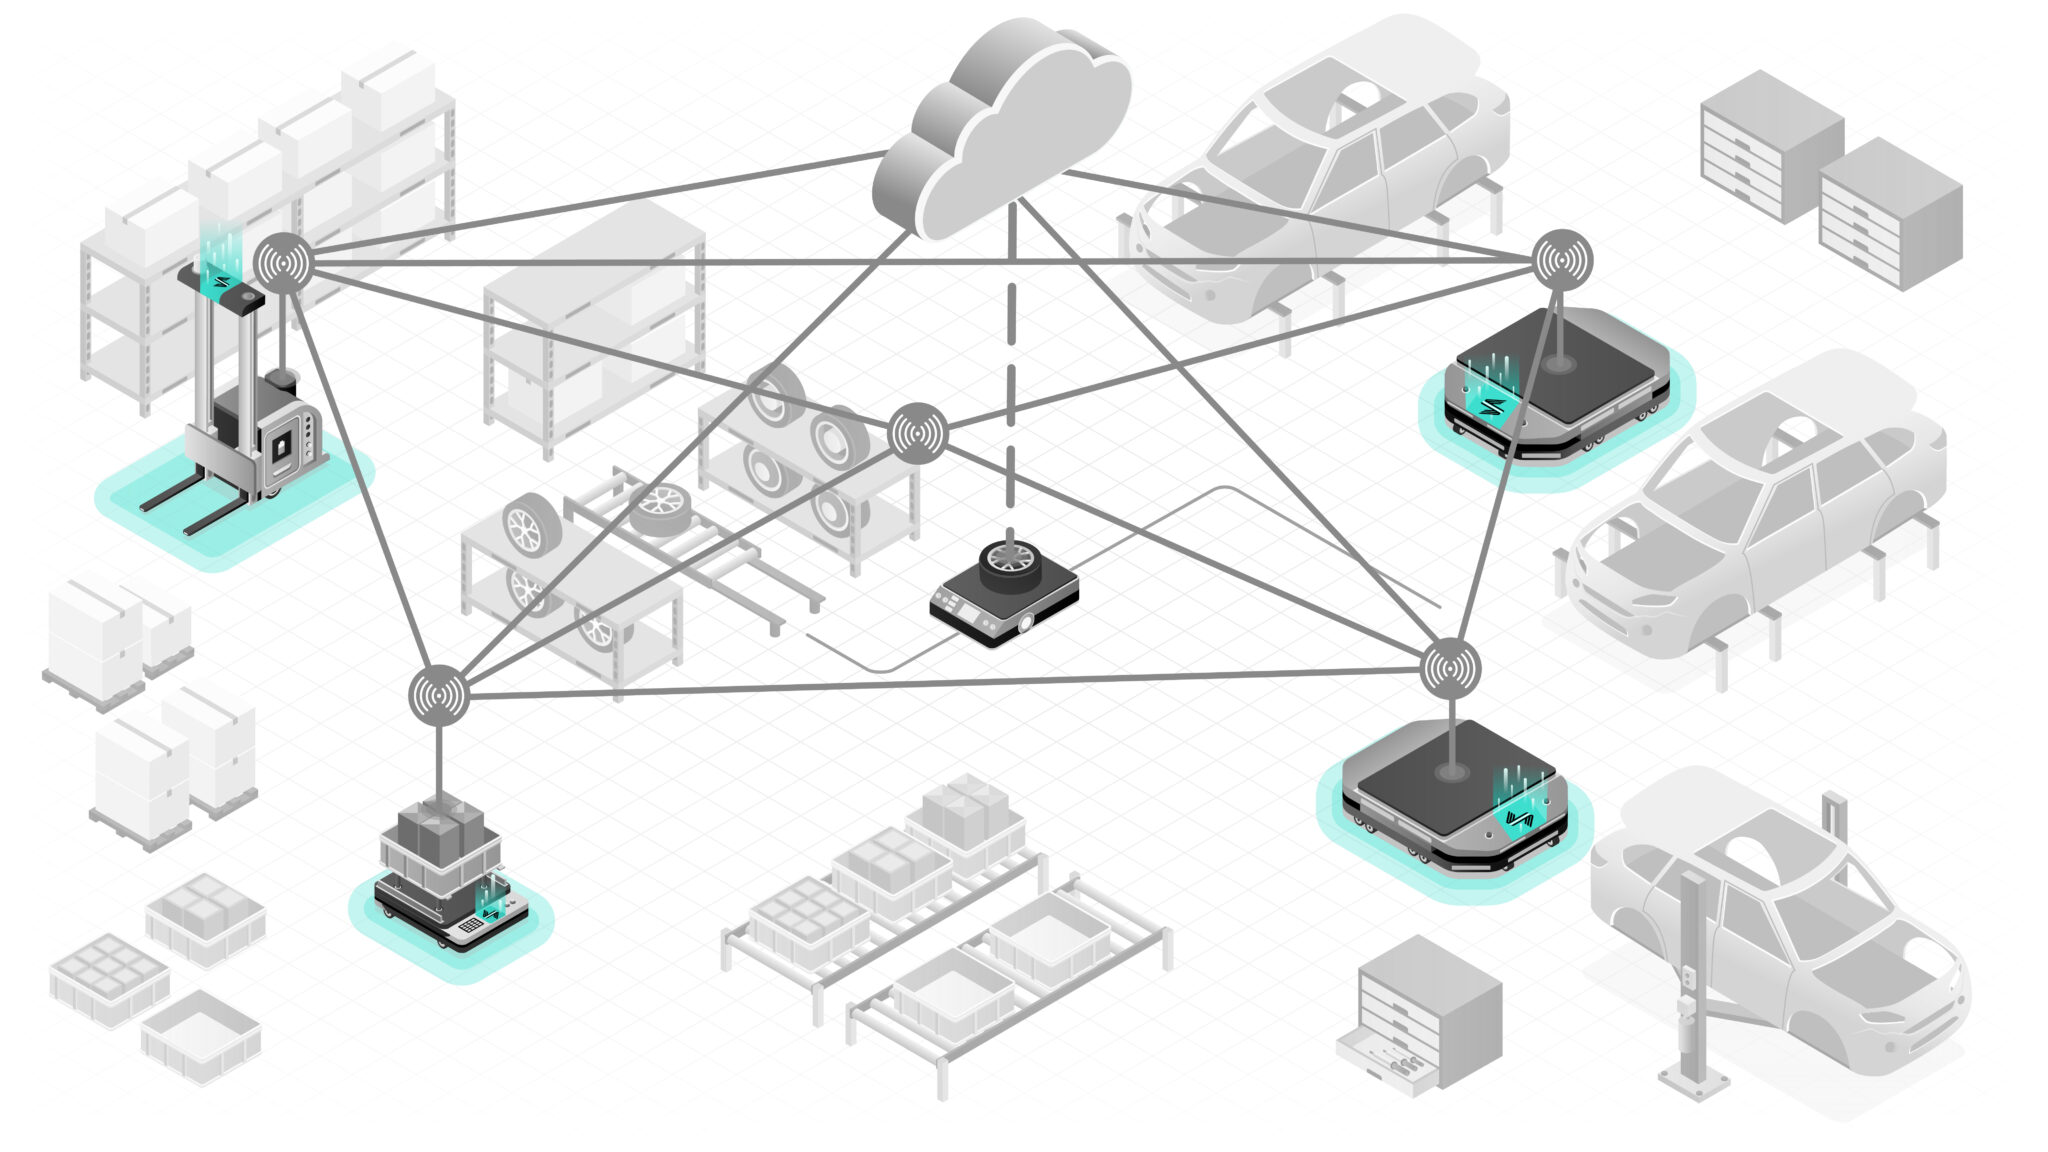
\includegraphics[height=9 cm]{images/structure.jpg}
		\caption{Basic capability of AMR for autonomous navigation}
	\end{center}
\end{figure}

Fleet management includes the inter-communication between robots and collaboration in path planning for multiple robots. 

To achieve both Autonomous navigation and fleet management with modularity, NODE provides four different components which are as listed
\begin{enumerate}
	\item NODE.OS
	\item NODE.EDGE
	\item NODE.MESH
	\item NODE.SRVS
\end{enumerate}

\subsection{NODE.OS}
NODE.OS is based on three independent but aligned software modules.
\subsection{NODE.EDGE}
NODE.EDGE is the software component which runs at the robot level. This software is used by the individual AMR to plan the path and navigate itself to the desired destination. This also includes the static obstacle avoidance. Continuously updated environment and data models enable the NODE.EDGE to adapt to environmental changes in real time and to cope with unforeseen situations. If desired, the AMRs avoid obstacles such as other vehicles or people and successfully execute even previously unknown orders.
\subsection{NODE.MESH}
NODE.MESH is the software component which helps for the collaboration of multiple AMR's. This includes obstacle avoidance dynamically and communicating between the robots will also ensures the shortest path without obstacles.
image here

\begin{figure}[h]
	\begin{center}
		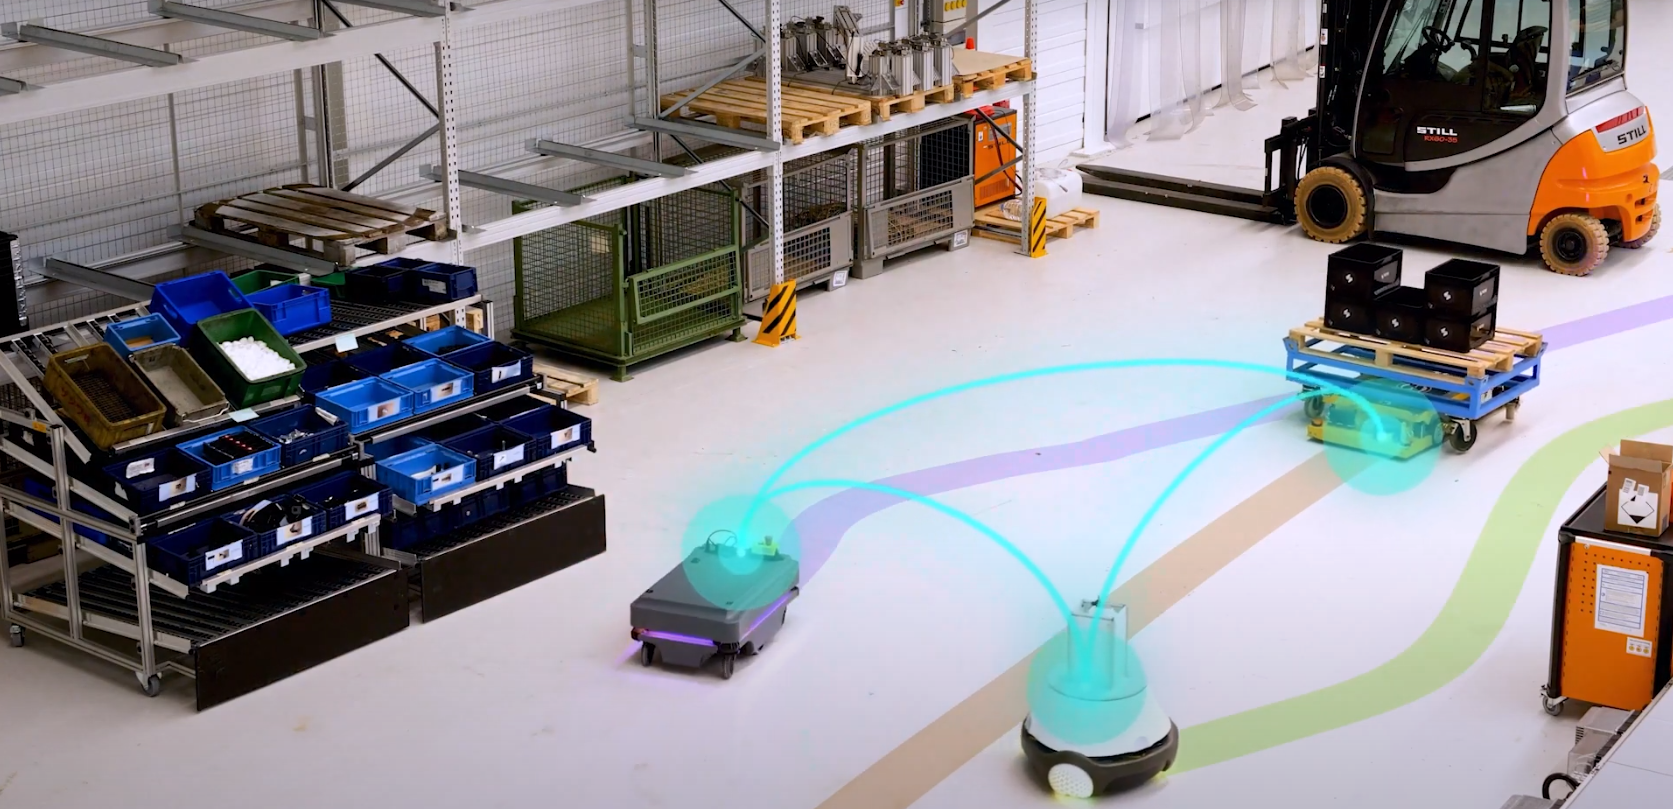
\includegraphics[height=5cm]{images/mesh.png}
		\caption{Collaboration of robots}
	\end{center}
\end{figure}
\subsection{NODE.SRVS}
NODE.SRVS will deals with cloud level fleet management and coordination of robots.

\vspace{0.5cm}
As an interface the VDA5050 standards are used along with Open API, to realize the autonomous fleets

\pagebreak
\section{Different teams of the company}
NODE Robotics has four different teams
\begin{enumerate}
	\item Perception and SLAM
	\item Fleet management system(FMS)
	\item Operations
	\item UI/UX

\end{enumerate}
\subsection{Perception and SLAM}
 This teams works with the mapping of the surrounding environment. Simultaneous localization and mapping will help the robot to localize itself inside the map. This part will also take care of creating the map from the LIDAR scanners. Basically main aim is to achieve the fastest localization of the robot in the current environment with matching the scans and obstacles present in the map. Also this team aims at creating the dynamic map based on inputs provided from the multiple robots.

\subsection{Fleet management system(FMS)}
Fleet management team works basically with the traffic management of the multiple robots. This team works with planned execution of mission and managing fleets. The Fleet Management System is a software package for transport mission of AGV's. On the plant operation side, this is achieved by exposing a unified REST-API for submitting POI's and also zones for traffic management.
\subsection{Operations}
Operations team work as bridge between the implementation of the algorithm and executing on the robot. This team also try to implement the backend like FMS stuff all on docker, so that implementation is easy and can be implemented everywhere without any implementation restriction. Also helps as the backend support for the frontend UI/UX department.
\subsection{UI/UX}
This team helps in visualizing the robots and map on the own frontend side. This helps in visualizing the robots, path and dedicated zones for the robots. This team is also trying to do the 3D representation of the robots and environment of the working area.

The following image in Figure 1.4 shows the appearance of NODE own frontend tool along with the robots and there path. In this same picture we can see some point names like south\_corner2 which indicates the point of interest. 

\begin{figure}[h]
	\begin{center}
		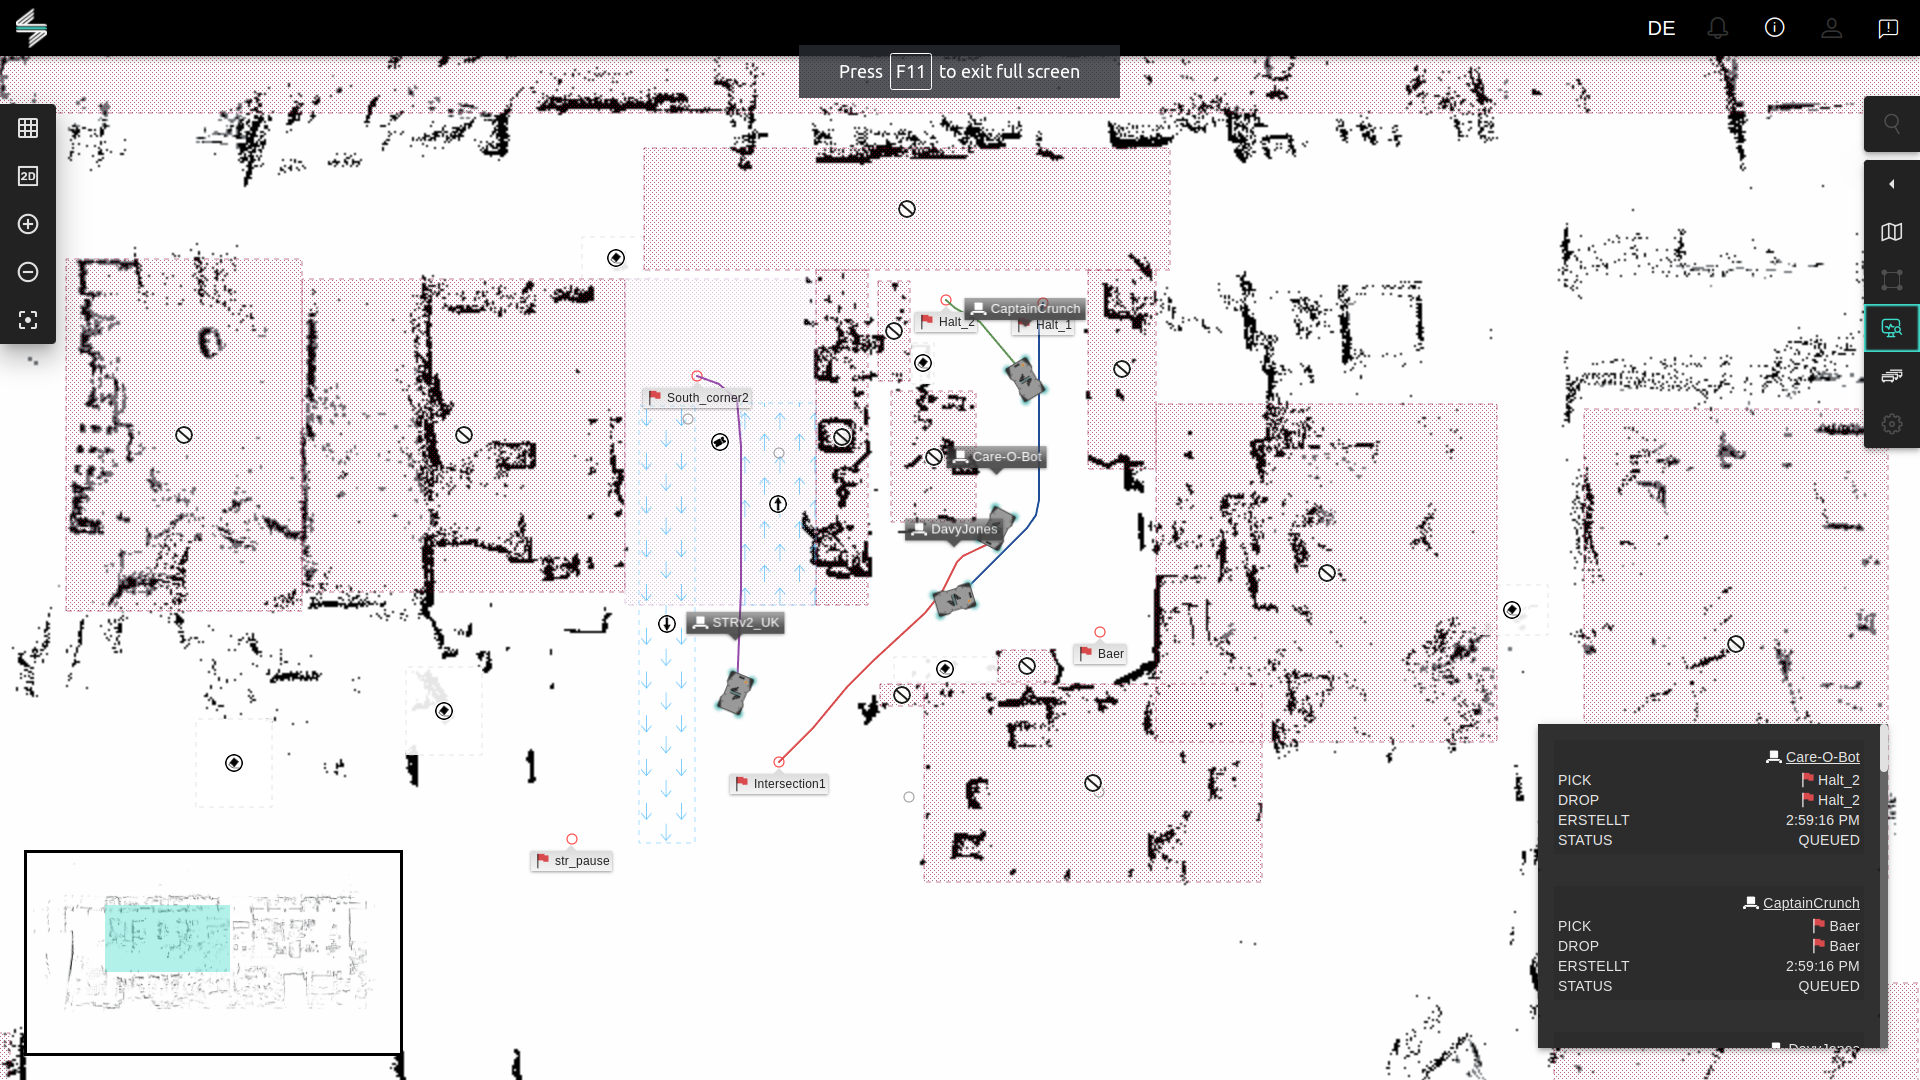
\includegraphics[height=10cm,width=\linewidth]{images/ui_ux.png}
		\caption{Frontend look of Fleet management product of NODE}
	\end{center}
\end{figure}

\section{About robots}
As mentioned NODE solutions are Industrial proof and they are tested for factory environment. This testing will be done on the robots that are available. Before every product release to the customers the release will be tested thoroughly with the available robot. These robots are also used to test any research or new ideas. Here is some of list of robots and their description.

	

\begin{wrapfigure}{r}{0.5\textwidth}
	\centering
	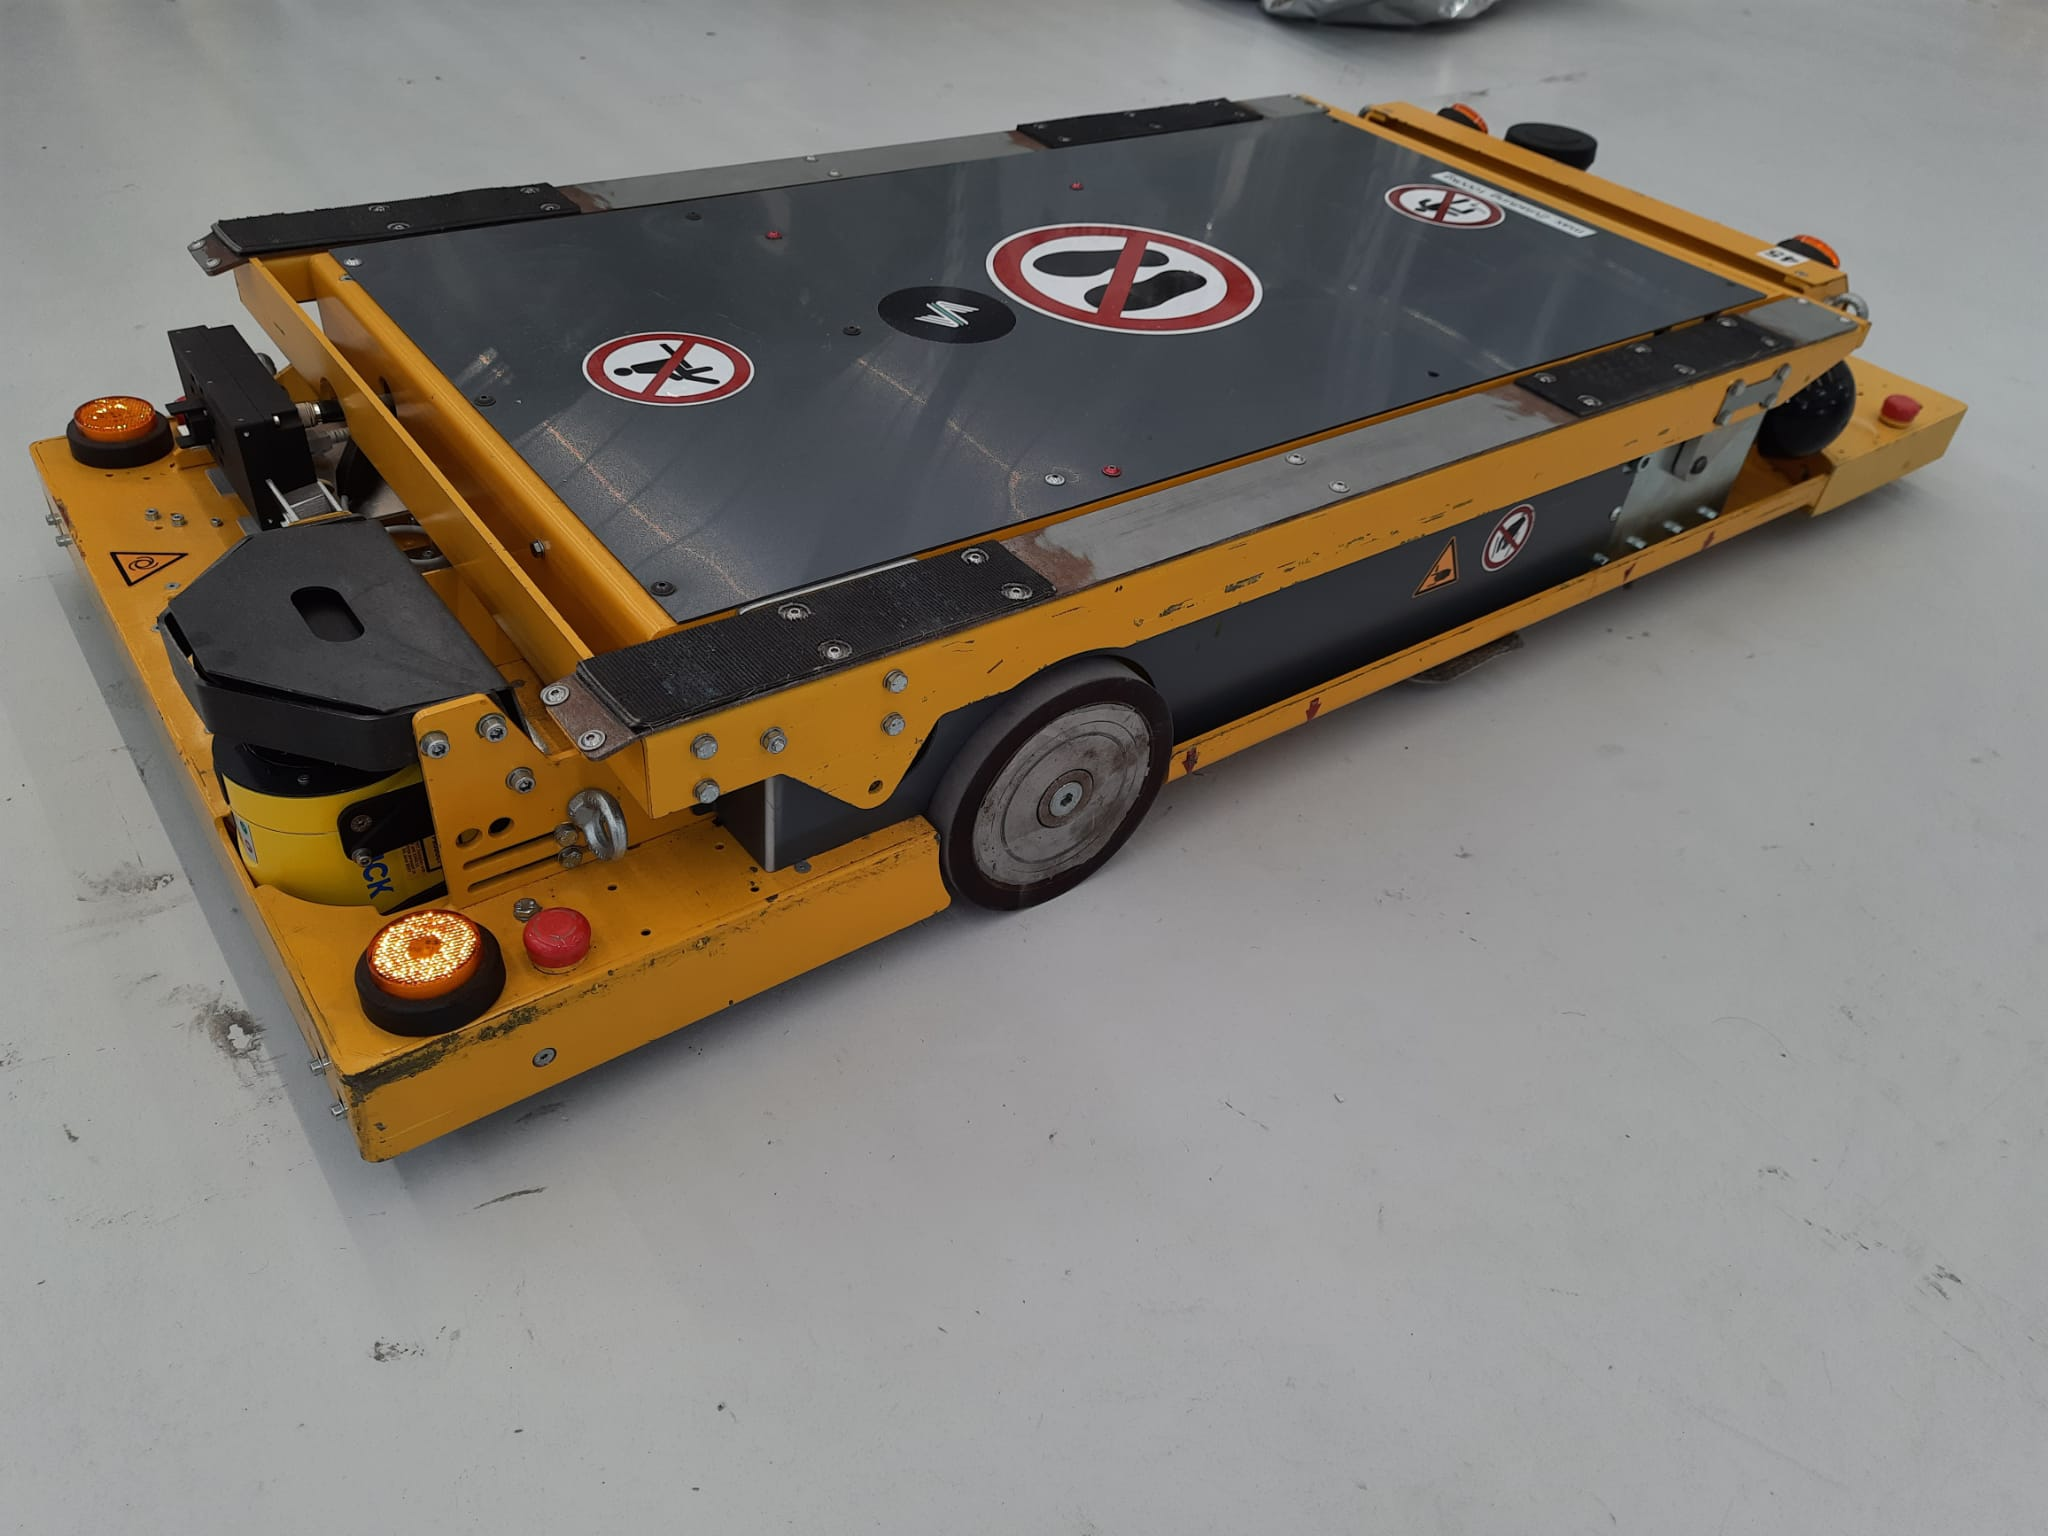
\includegraphics[width=2cm,height=2cm]{images/str.jpeg}
	\caption{STR robot}
\end{wrapfigure}
\subsection{BMW-STR:}
STR are mainly \hspace{2cm}used for the\hspace{2cm} production house in BMW warehouse. This is mainly used \hspace{2cm}to test the releases for the\hspace{2cm} BMW. This robot can lift tons of weight. 

Apart from the str we can also find two different series of Mobile-industrial-robots(MIR)


\begin{wrapfigure}{l}{0.5\textwidth} 
	\centering
	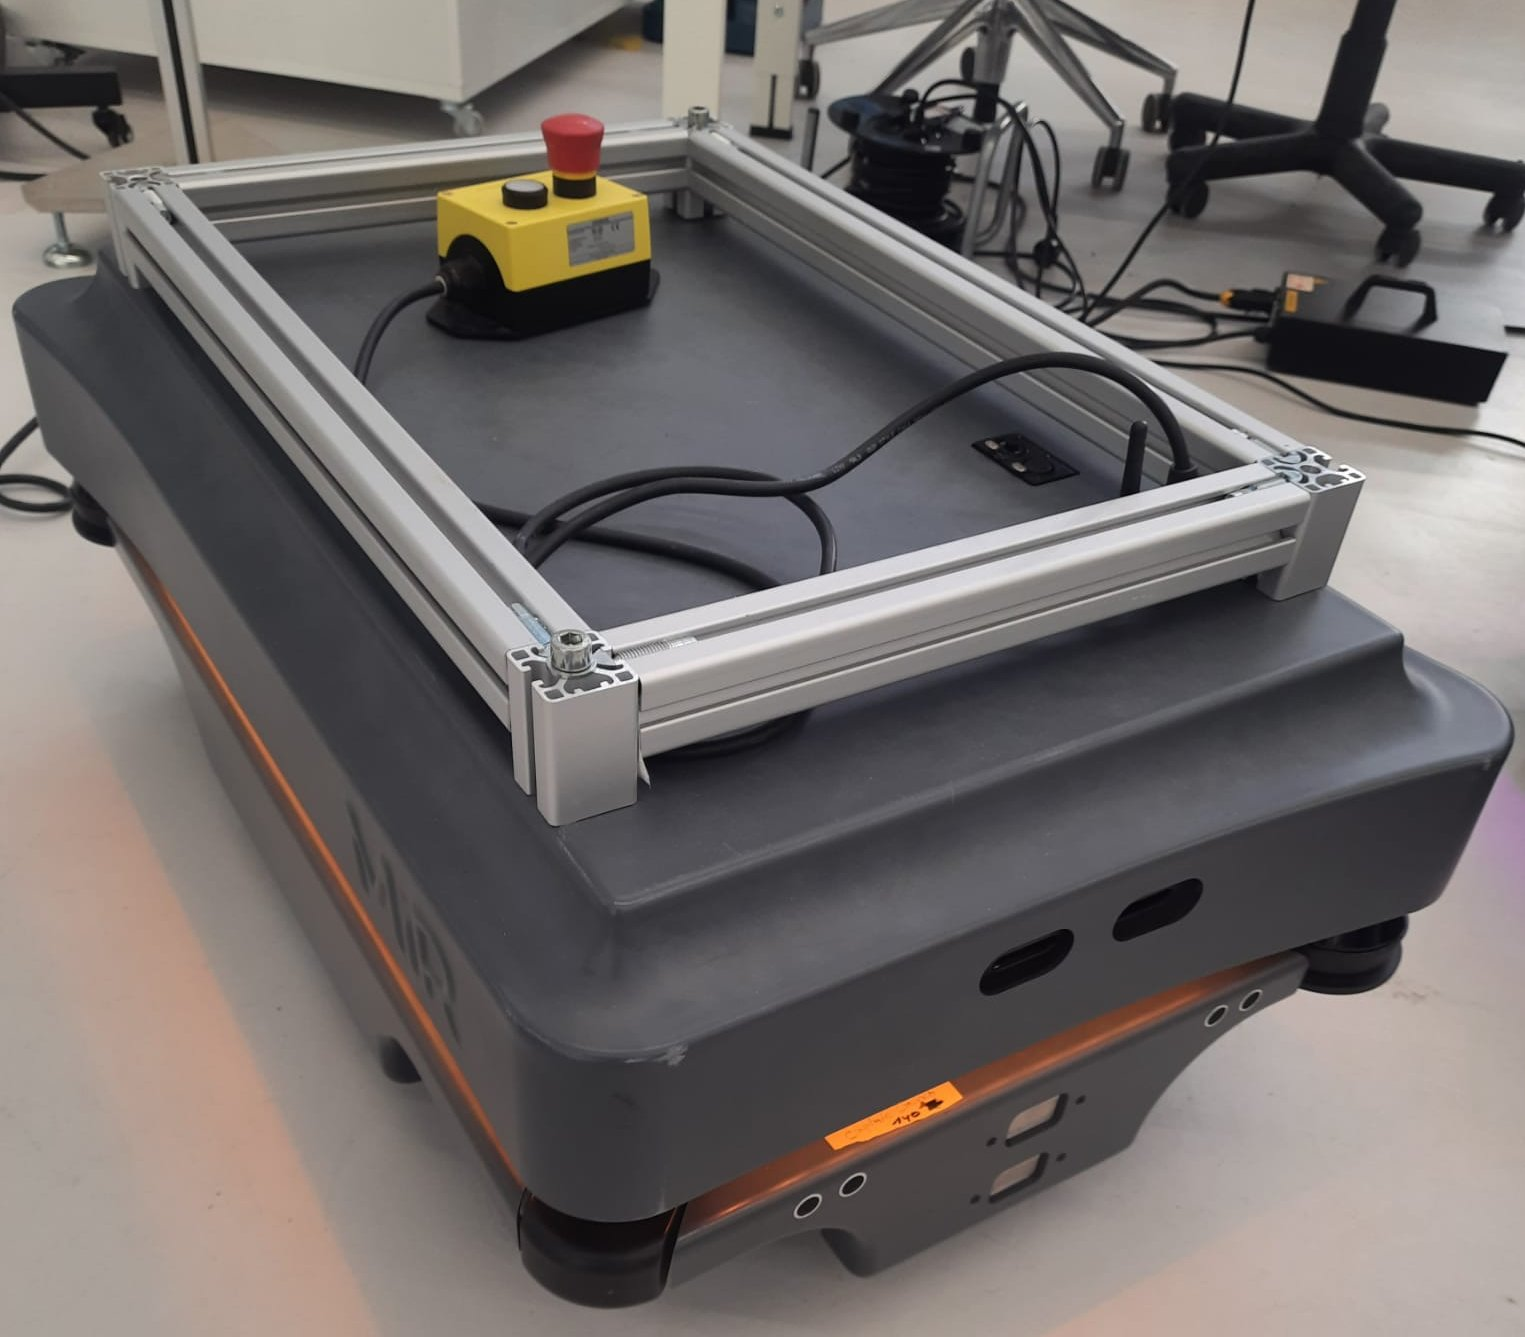
\includegraphics[width=2.5cm,height=2.5cm]{images/mir1.jpeg}
	\caption{mir100 robot}
\end{wrapfigure}
\subsection{MIR100:}
MiR which is known as Mobile industrial robots. This has the maximum speed of 1.5m/s, which can carry up to 100 kg of load. This robot is most suitable for indoor operations. This robot has four ultrasound sensors, two SICK safety laser scanners(front and rear).
	

\begin{wrapfigure}{r}{0.5\textwidth}
	\centering		
	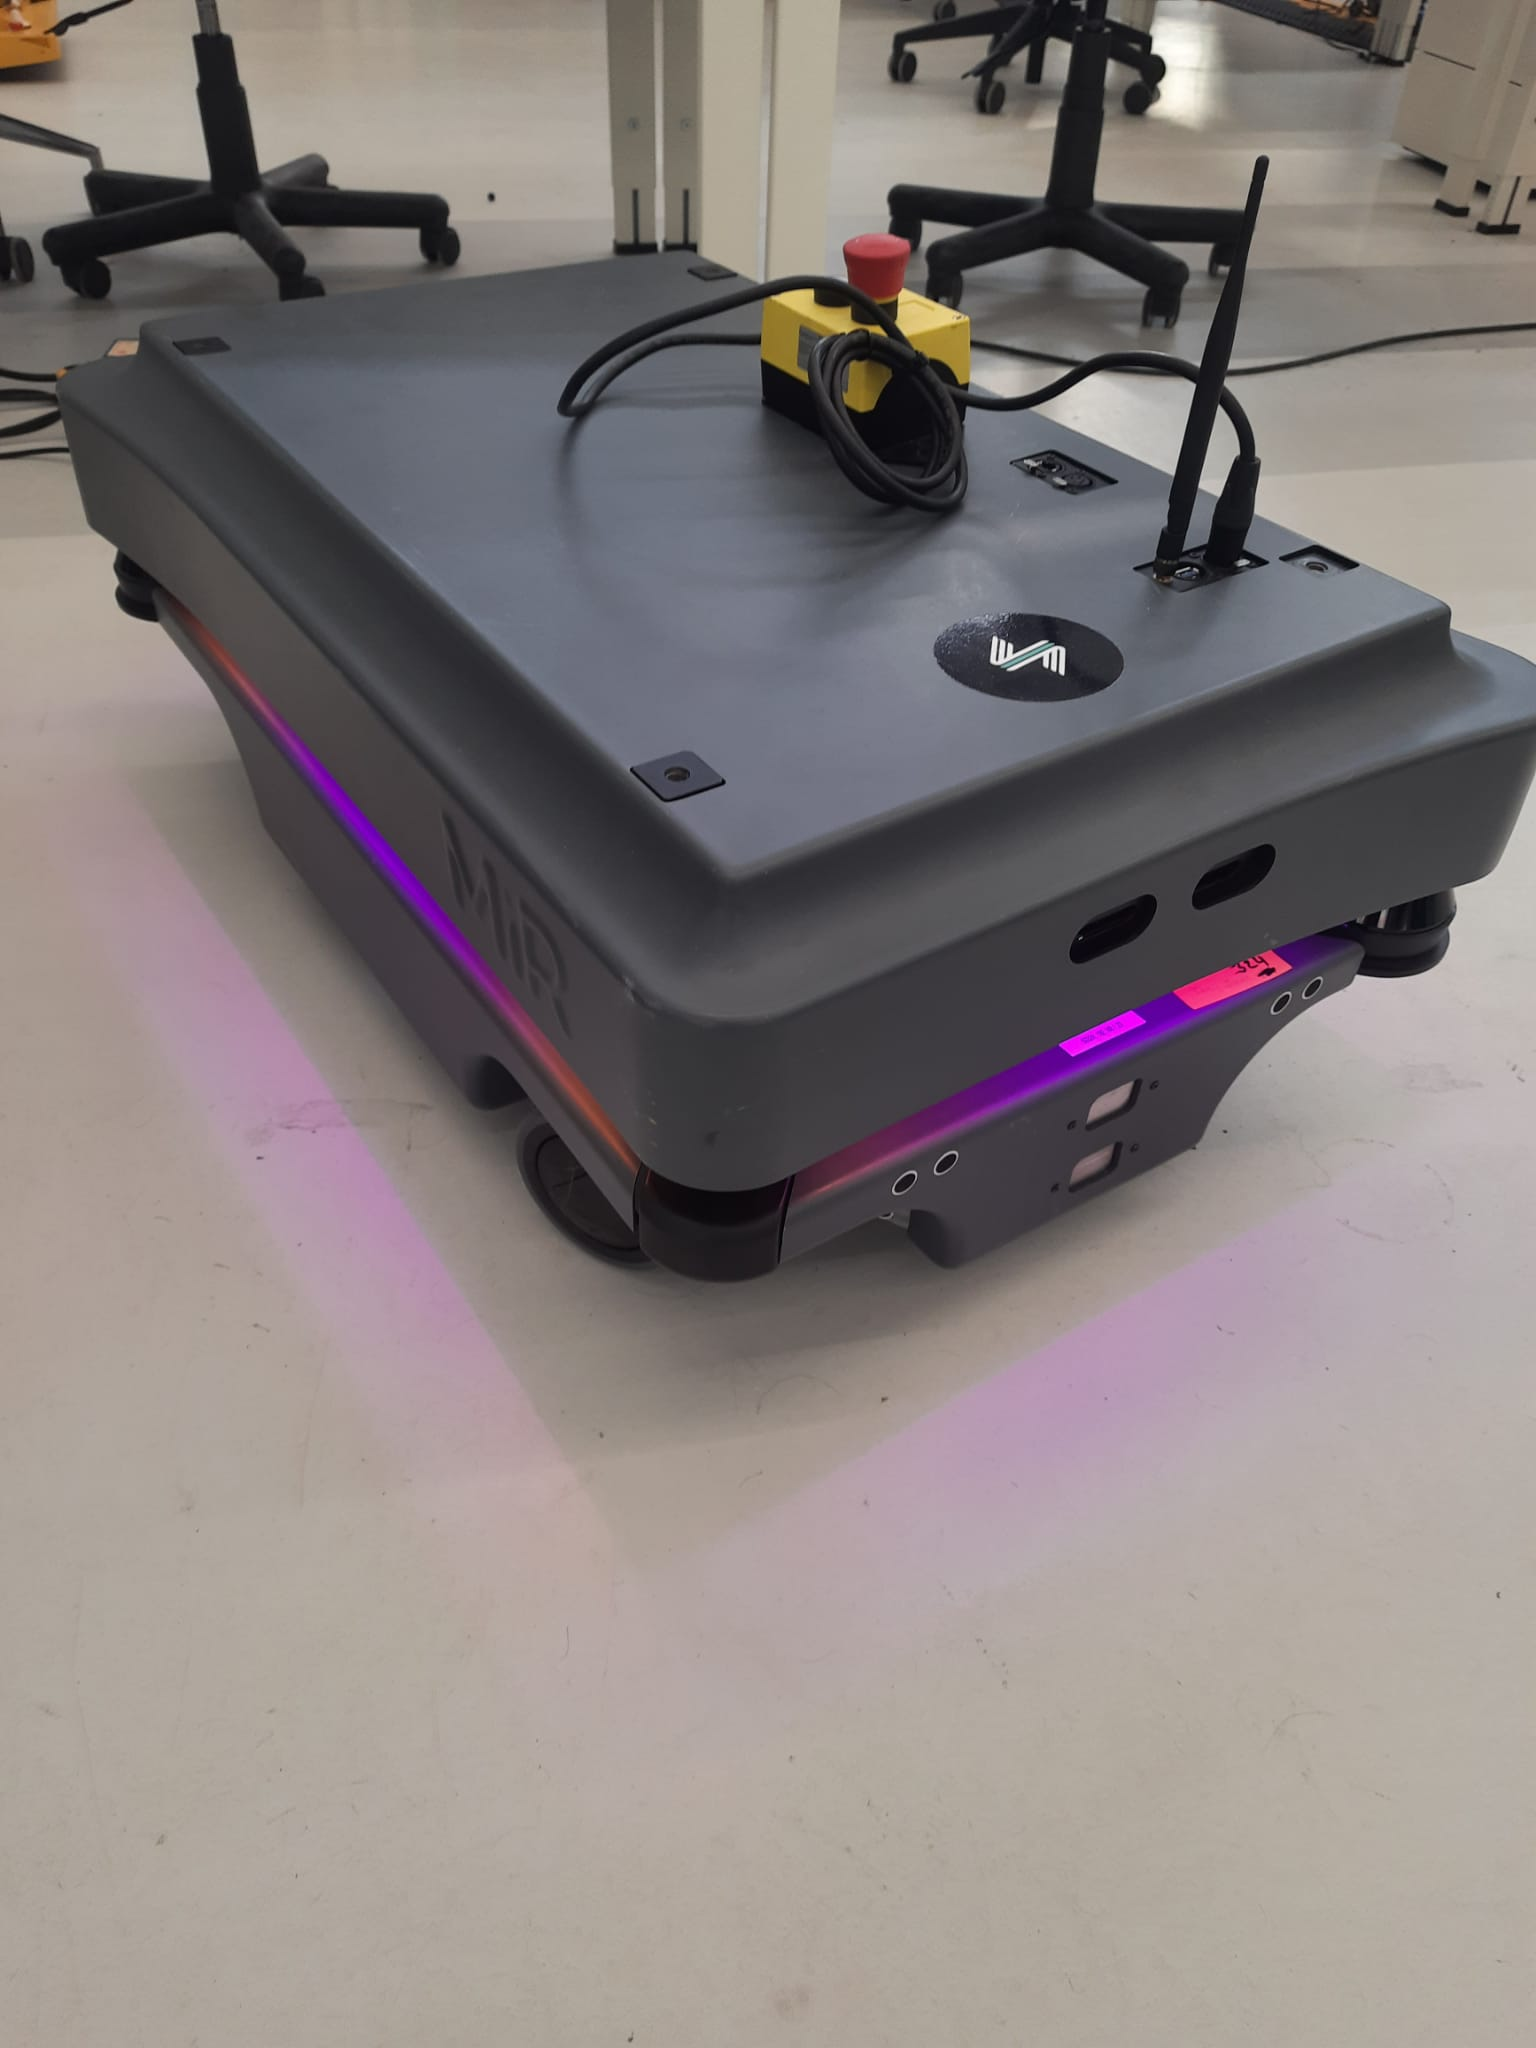
\includegraphics[width=2.5cm,height=2.5cm]{images/mir2.jpeg}
	\caption{mir200 robot}
\end{wrapfigure}
\subsection{MIR200:}	
This robot is a slightly updated version of MIR100. This has the maximum speed of 2.0ms, Payload of 250 kg. This has also feature called over-speed avoidance which prevents the robot from driving faster than predefined safety limit. Safety sensors wise it has same configuration as MIR100.


\begin{wrapfigure}{l}{0.5\textwidth} %this figure will be at the right
	\centering
	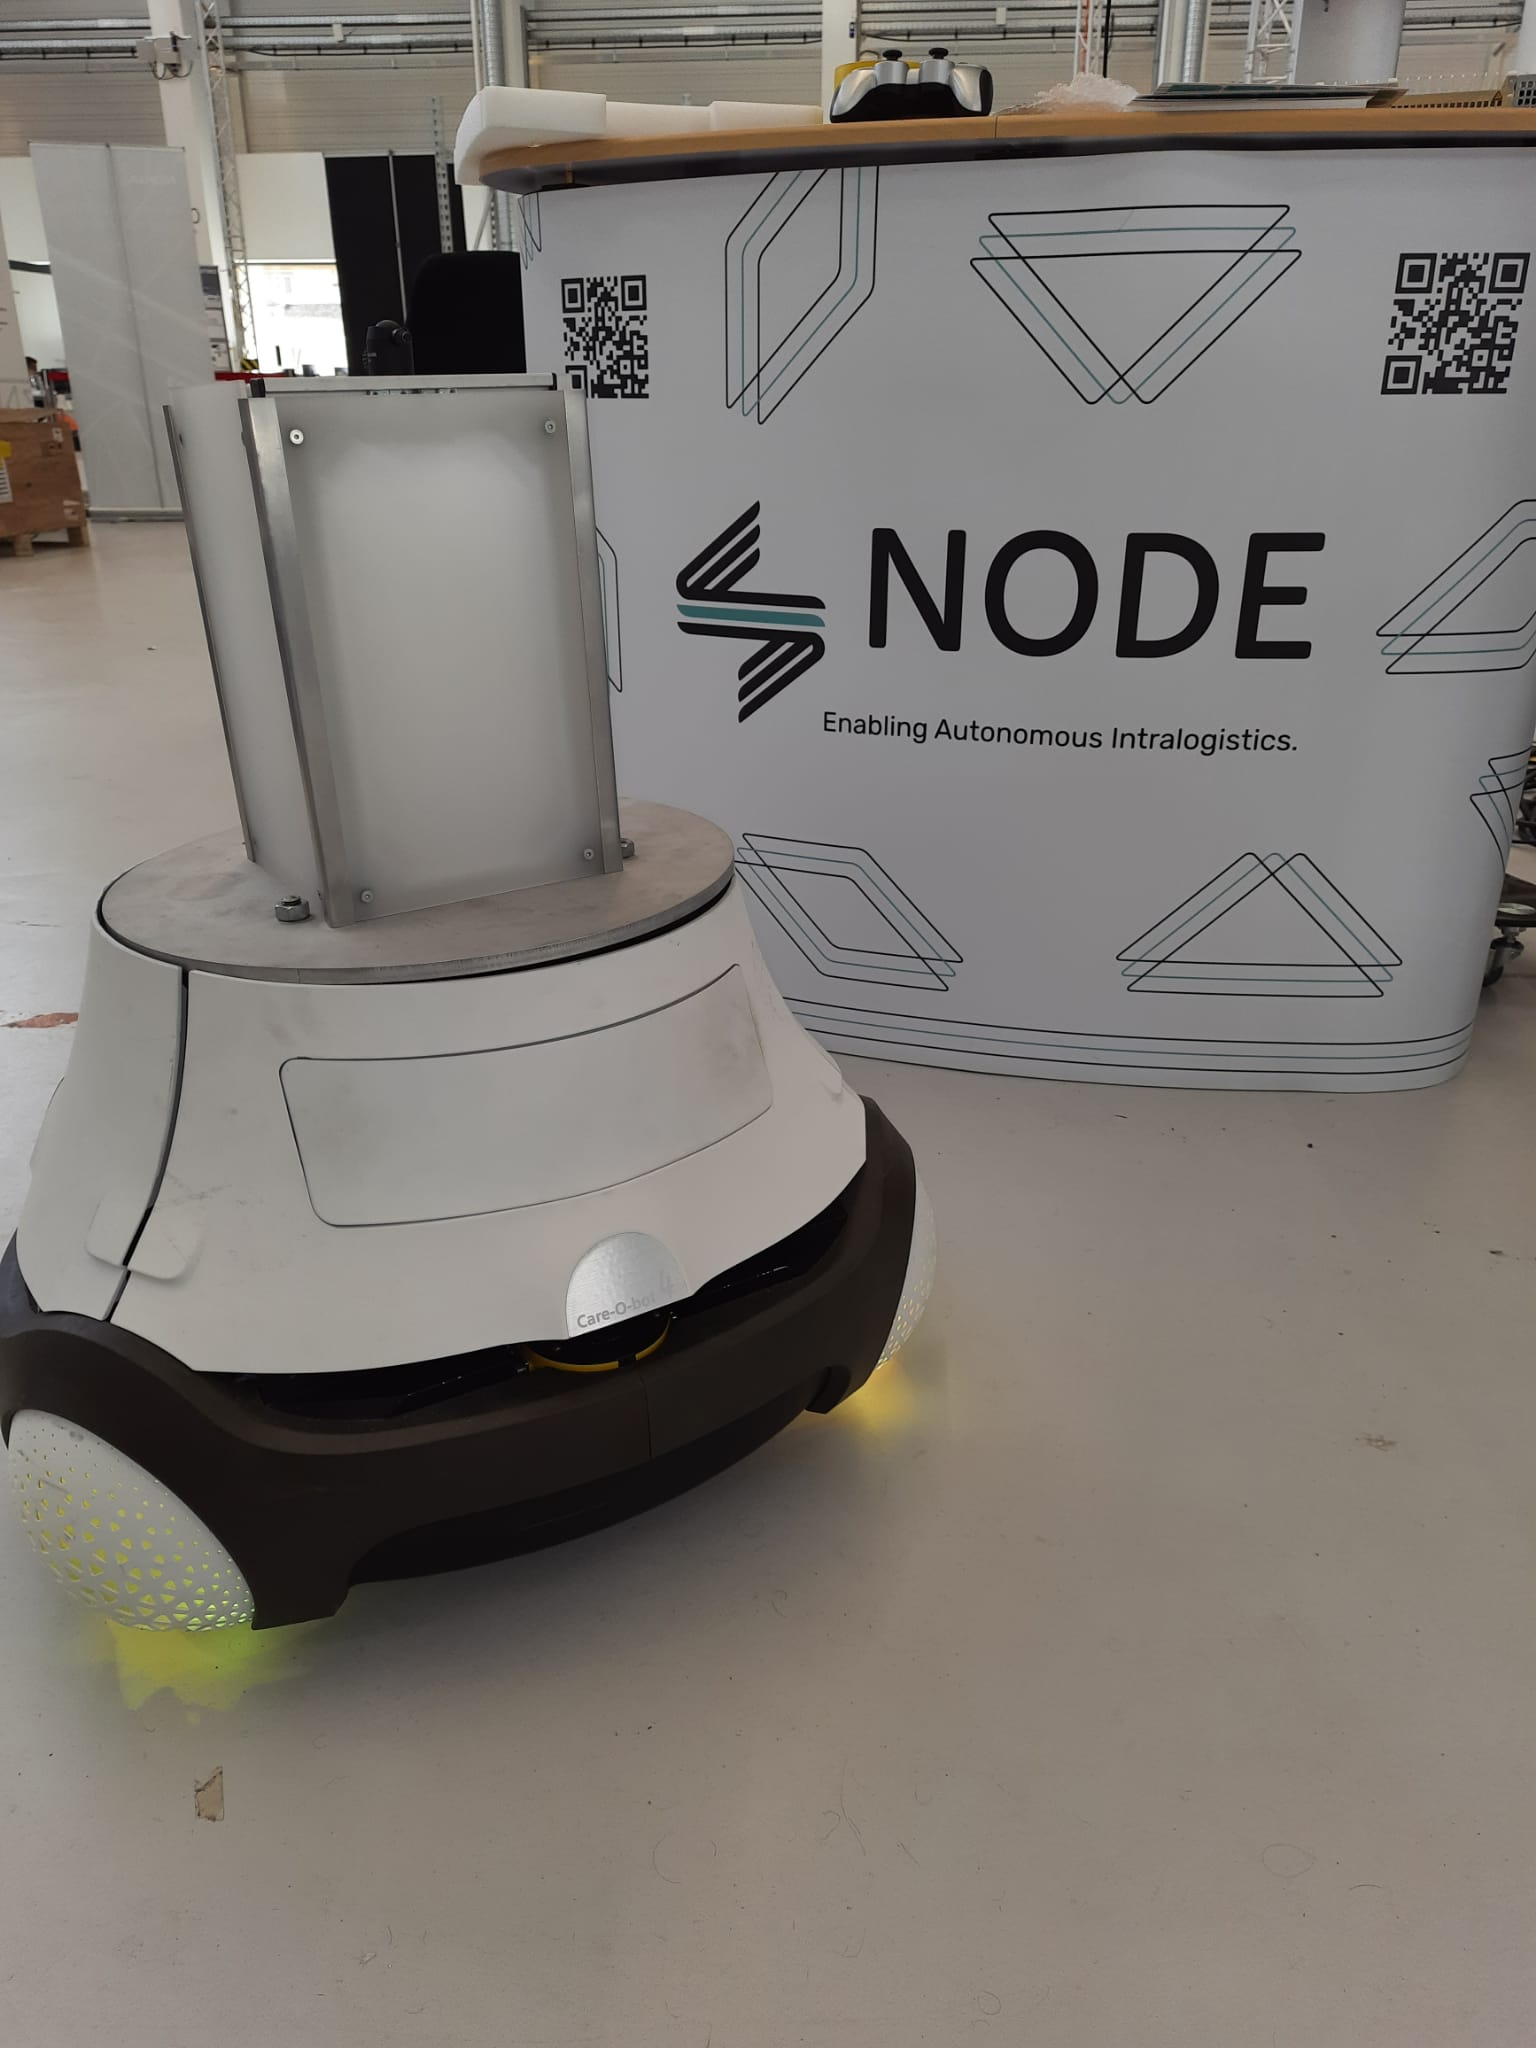
\includegraphics[width=2.5cm,height=2.5cm]{images/cob.jpeg}
	\caption{Care-o-bot}
\end{wrapfigure}
\subsection{Care-O-Bot:}
Care-O-bot is the product vision of a mobile robot assistant to actively support people in the home environment. This robot is omni-directional robot with three wheels. Since the NODE robotics only focusses on the research and development regarding the navigation and fleet, therefore only the lower body of cob is present.
	

With the above robots the operational setup will be done to give some operational demos to some of the companies. This will also be used for research and development.

\begin{figure}[h]
	\begin{center}
		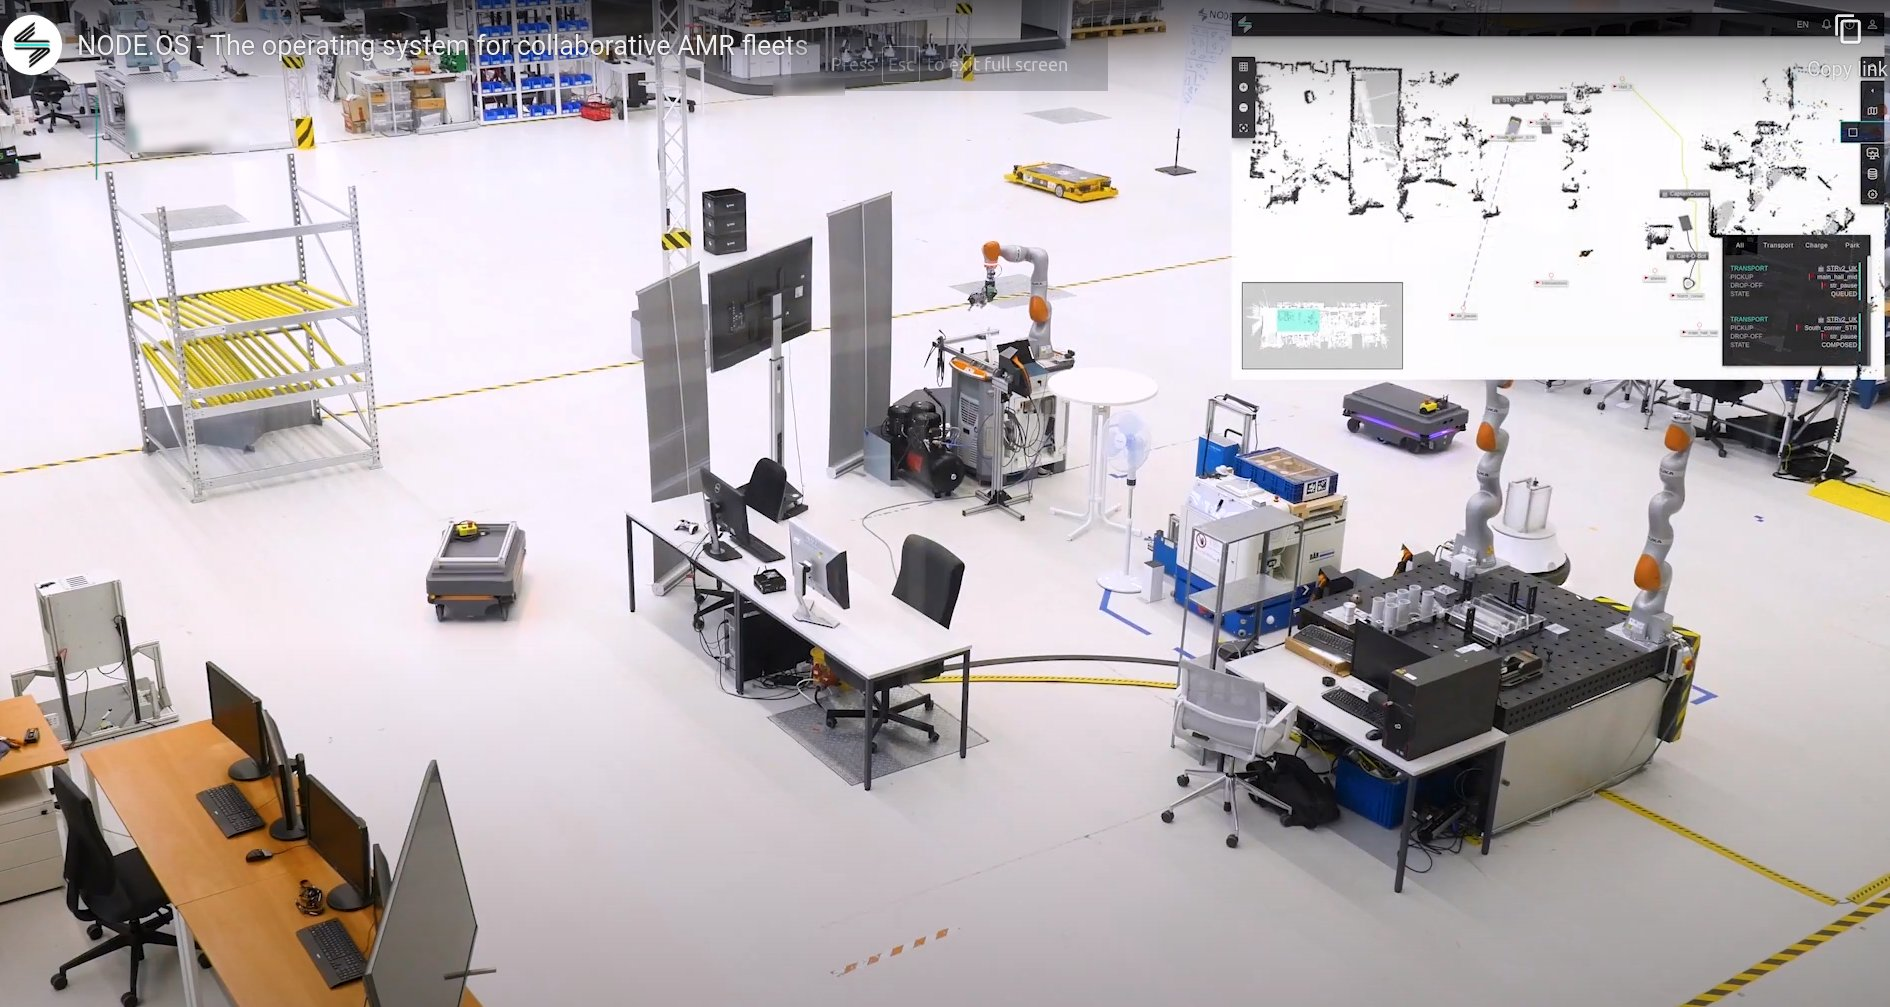
\includegraphics[height=10cm,width=\linewidth]{images/operation.jpg}
		\caption{Workspace of NODE robotics}
	\end{center}
\end{figure}

\pagebreak
\section{Problem statement and research objectives}
\subsection{Problem statement}
As discussed before I worked on a project of developing a UI for rosbag analysis. This was basically part of on-going BMW project. There was a requirement to develop a User-interface which basically analyze the given recorded rosbag. I was given opportunity to support on the backend side of this project. Basically the frontend part like visualizing the robots is basically done by UI-fronend team. We on the backend side should make sure that ROS part works along the frontend. Basic requirements were to play the bag just like playing the video. This included speeding the ROSBAG, stepping to the particular location, loading of rosbag to the cloud, stopping of rosbag. All this has to be done using rosservice call. 

\subsection{Desired outcome}
I was involed in the research of suitable python libraries that can be used to manipulate the rosbag. In this project we must be able to call the rosservice and rostopics using web-sockets. Therefore the communication protocol between the frontend and backend should be done via web-sockets. Also we must use the rosbridge for the communication. 
\subsection{Organization of report}
The report is organized as follows. Chapter 2 will give a brief background of the technical topics that is required to understand this report. This also explains about used during entire internship. Chapter 3 explains about the concept implemented during the internship. This explains why particular concept is chosen to implement the project. Next in Chapter 4 explains the final result of the project. Chapter 5 deals with the various methods that is used to verify and validate the results. Finally chapter 6 gives the final conclusion and future scope.

	\chapter{Technical Background}

\section{ROS}

The Robot Operating System (ROS) is a flexible framework for writing robot software. It is a collection of tools, libraries, and conventions that aim to simplify the task of creating complex
and robust robot behavior across a wide variety of robotic platforms. 

ROS is an open-source, meta-operating system for your robot. It provides the services you would expect from an operating system, including hardware abstraction, low-level device control,
implementation of commonly-used functionality, message-passing between processes, and package management. It also provides tools and libraries for obtaining, building, writing, and running code across multiple computers.

The ROS runtime "graph" is a peer-to-peer network of processes (potentially distributed across
machines) that are loosely coupled using the ROS communication infrastructure. 
ROS implements several different styles of communication, including synchronous RPC-style communication over services, asynchronous streaming of data over topics, and storage of data
on a Parameter Server.

ROS is a distributed framework that enables executable to be individually catered and tailored
based on the needs of the developer and the design of the application. ROS also supports docker
platform for the ease of virtualization and deliver software in terms of Containers[2].

\begin{figure}[h]
	\begin{center}
		
\includegraphics[height=2.5cm]{images/ros_logo.png}
		\caption{ROS logo}
	\end{center}
\end{figure}


\section{Rosbag}

This is a set of toll which is used to playing and recording of the ROS topics. It is basically used for high performance and avoids de-serialization and re-serialization of the messages. Bags are a format for saving and playing back ROS message data. Bags are an important mechanism for storing data, such as sensor data, that can be difficult to collect but is necessary for developing and testing algorithms[3]. 

\section{Rosbridge}


Rosbridge makes ROS topics and services available over either pure TCP sockets or web-sockets as JSON messages. Rosbridge provides a JSON API to ROS functionality for non-ROS programs. There are a variety of front ends that interface with rosbridge, including a WebSocket server for web browsers to interact with. Rosbridge\_suite is a meta-package containing rosbridge, various front end packages for rosbridge like a WebSocket package, and helper packages[4].

\section{Websockets}

WebSocket is a computer communications protocol, providing full-duplex communication channels over a single TCP connection. The WebSocket protocol was standardized by the IETF as RFC 6455 in 2011, and the WebSocket API in Web IDL is being standardized by the W3C.


Unlike HTTP, WebSocket provides full-duplex communication.[5] Additionally, WebSocket enables streams of messages on top of TCP.


\section{REST-API}

A REST API (also known as RESTful API) is an application programming interface (API or web API) that conforms to the constraints of REST architectural style and allows for interaction with RESTful web services. REST stands for representational state transfer[5].

An API is a set of definitions and protocols for building and integrating application software. It’s sometimes referred to as a contract between an information provider and an information user—establishing the content required from the consumer which is referred as call and the content required by the producer as the response.
\pagebreak
\section{REST-API v/s Websockets}
In this section there is comparison between the REST-API and WebSockets
\begin{table}[!htbp]
\centering
\resizebox{\columnwidth}{2.5cm}{\begin{tabular}{|c|c|c|}
	\hline
	\textbf{The basis of Comparison}& \textbf{WebSocket}  & \textbf{REST-API}  \\
	\hline
	\textbf{HTTP}&The use of HTTP occurs in the initial connection.  & HTTP is a common protocol in RESTful web services. \\
	\hline
	\textbf{Communication}& Bi-directional  & Uni-directional \\
	\hline
	\textbf{Nature}& Socket-based & Resources based concept, rather than commands \\
	\hline
	\textbf{Scenario}& Real time and continuous communication  & Based on the service request \\
	\hline
	\textbf{Dependency}& IP address and port number & Based on HTTP protocol \\
	\hline
	\textbf{Cost}& Cost of communication is lower & The cost of communication is slightly higher that WebSockets  \\
	\hline
	\textbf{Performance}& Better with high loads & Great for occasional communication \\
	\hline
	\textbf{State}& Websocket is a stateful protocol & REST is based on HTTP, which is a stateless protocol. \\
	\hline
\end{tabular}}
\caption{Comparison of WebSocket and REST-API}
\end{table}

\section{RViz}

RVIZ is a ROS graphical interface that allows you to visualize a lot of information, using plugins for
many kinds of available topics. It is a powerful robot visualization tool. It provides a convenient GUI to
visualize sensor data, robot models, environment maps, which is useful for developing and debugging
your robot controllers. It provides a view of your robot model, capture sensor information from robot
sensors, and replay captured data. It can display data from camera, lasers, from 3D and 2D devices
including pictures and point clouds.

It is designed to visualize data from the ROS framework. It also runs as a ROS node that can subscribe
to topics and display the contents of these messages. This is mainly used to display sensor data, like
point cloud data from a LiDAR or infrared distance measurements that are published to this topic by the
sensor.

It was used to visualize published information from the robot and also used in a later stage to issue
commands to the robot for navigation purposes. The software was chosen because of its tight
integration with the ROS framework. Rviz makes use of a file format called Universal Robotic
Description Format (URDF). A URDF file describing the Tiago was used to describe the robot and its
capabilities to Rviz. URDF files are written in XML by using the macro language xacro. This made the
URDF files easier to maintain and to read.

ROS makes use of topics to send messages from a publisher to a subscriber. Gazebo published
simulation messages which were computed within the ROS framework and then published to Rviz for
visualization. 


\section{Docker}

Docker is a open platform for developing, shipping and running application. Docker helps to run the developed application to run independent of the infrastructure used to develop. All the application will run on the docker cloud platform. Hence it will be independent of the underlying OS.

\subsection{Docker architecture}
Docker uses a client-server architecture[8]. The Docker client talks to the Docker daemon, which does the heavy lifting of building, running, and distributing your Docker containers. The Docker client and daemon can run on the same system, or you can connect a Docker client to a remote Docker daemon. The Docker client and daemon communicate using a REST API, over UNIX sockets or a network interface. Another Docker client is Docker Compose, that lets you work with applications consisting of a set of containers.

\begin{figure}[h]
	\begin{center}
		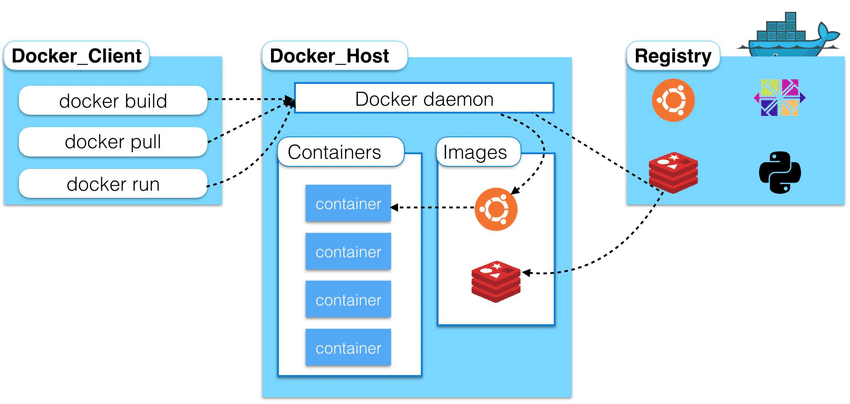
\includegraphics[height=10 cm,width=\linewidth]{images/docker_architecture.png}
		\caption{Docker Architecture}
	\end{center}
\end{figure}

\subsection{Docker objects}

When using Docker, we are creating and using images, containers, networks, volumes, plugins, and other objects. This section is a brief overview of some of those objects.


\onecolumn
\textbf{Images}

An image is a read-only template with instructions for creating a Docker container. Often, an image is based on another image, with some additional customization. For example, building an image which is based on the ubuntu image, but installs the Apache web server and our application, as well as the configuration details needed to make our application run.

We can also create our own images or we might only use those created by others and published in a registry. To build our own image, we create a Dockerfile with a simple syntax for defining the steps needed to create the image and run it. Each instruction in a Dockerfile creates a layer in the image. When we change the Dockerfile and rebuild the image, only those layers which have changed are rebuilt. This is part of what makes images so lightweight, small, and fast, when compared to other virtualization technologies.


\textbf{Containers}

A container is a runnable instance of an image. We can create, start, stop, move, or delete a container using the Docker API or CLI. We can connect a container to one or more networks, attach storage to it, or even create a new image based on its current state.

By default, a container is relatively well isolated from other containers and its host machine. You can control how isolated a container’s network, storage, or other underlying subsystems are from other containers or from the host machine.

A container is defined by its image as well as any configuration options you provide to it when you create or start it. When a container is removed, any changes to its state that are not stored in persistent storage disappear.

\section{VDA5050}

VDA 5050 is a standardized interface for AGV communication. Specifically, this standard concerns the communication between AGVs (often called Fahrerloser Transportsysteme/Transportfahrzeuge (FTS) in Germany) and a master control (in other words, a fleet management software program)[9].

In today's industries many AGV's of different manufacturers will be working together. Typically, these AGVs only work with their manufacturer’s own specific fleet management software. 

So some of the challenges arises in the industries such as

\begin{enumerate}
	\item Complex commissioning – a separate installation is needed for each brand of AGV
	\item Interoperability issues – it becomes difficult to manage AGVs if they need to cross paths or share an elevator say
	\item Lost space – separate AGV brands might need to use completely separate paths 
\end{enumerate}

Therefore VDA 5050 intends to provide a more generic version of this functionality, which would enable every compliant AGV to work together.

\begin{figure}[h]
	\begin{center}
		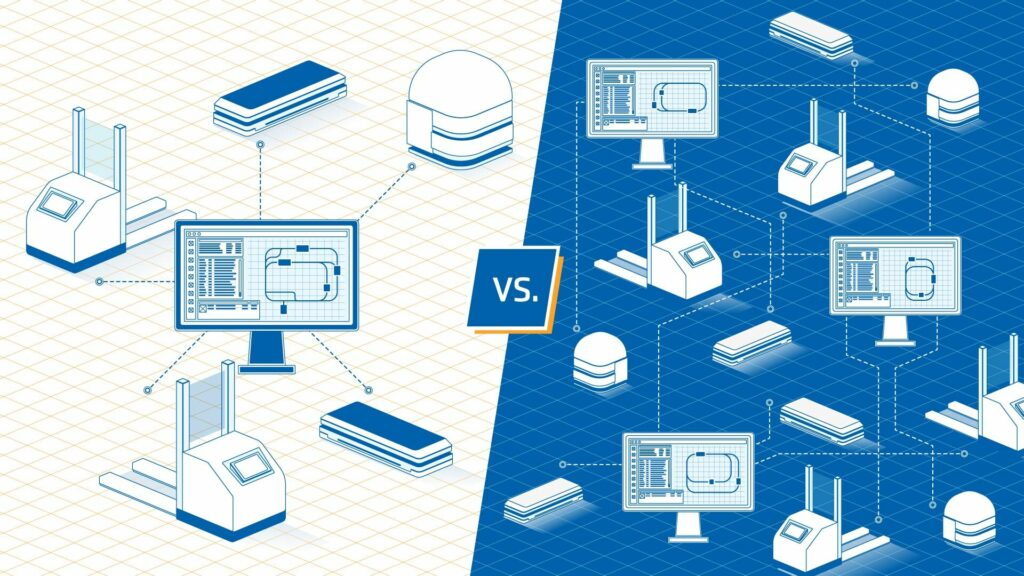
\includegraphics[height=10 cm,width=\linewidth]{images/vda.jpg}
		\caption{Main goal of VDA 5050 interface to bring most of the AMR in single Fleet}
	\end{center}
\end{figure}
\pagebreak
\section{CI/CD}

CI/CD is a method to frequently deliver apps to customers by introducing automation into the stages of app development. The main concepts attributed to CI/CD are continuous integration, continuous delivery, and continuous deployment. CI/CD is a solution to the problems integrating new code can cause for development and operations teams[10].

Specifically, CI/CD introduces ongoing automation and continuous monitoring throughout the lifecycle of apps, from integration and testing phases to delivery and deployment. Taken together, these connected practices are often referred to as a "\textbf{CI/CD pipeline}" and are supported by development and operations teams working together in an agile way with either a DevOps or site reliability engineering (SRE) approach.
\section{Webviz}

Webviz is a tool which is used to visualize the topics and messages that have been recorded in the ROSBAG. This tool is basically developed by Cruise Automation for visualizing the complex decision made by their vehicle both on road and in simulation. This tool provides the drag and drop feature of rosbag to analyze the data[6].

	\chapter{Concept implemented}
As per the requirements given by the BMW, idea is to implement a User-Interface which can be used to play the recorded rosbag with more clarification and detailed information display of some ros-topics which were required for understanding the errors and failure. This implementation is based on the idea of webviz tool, where the required rosbag is uploaded to the website and rosbag is played in that tool.

So in this project the approach was to send the HTML requests from the frontend webpage. The backend side will work with the ROS service call and topic. The communication protocol required between the frontend side and ROS will happen via websockets and rosbridge. In this project some of the functionalities like uploading of the rosbag to the cloud, getting information from the rosbag, for updating the information of environments of the factory is done using the REST-API tool.  

Basically playing the rosbag is considered as playing the video on video player. So the requirements were framed using that idea. The basic idea was to upload the bagfile to the cloud. Then we will select the bagfile to be analysed. This bagfile should be loaded in the backend using the ros-tools. Once the bagfile is loaded we must be able to play, pause and play the bagfile as many times, we must be able to step to the particular time in the rosbag using the slider. On the other we must also be able to manipulate the playback speed of the rosbag such that we can play with the required speed. 

Here as the rosbag is recorded in the different factories of the BMW, so map of factories will change. Since with the rosbag record we cannot take the map, so selecting of environments should be enabled. 

In BMW factories, movement of materials happens with str. Since they use different versions of str, so the detecting/selecting of robot is also feature needed to be implemented.

When the number of rosbag exceeds, the memory consumption also increases. So the logic to delete the old rosbag should also be implemented. As in the factory, it will be dynamic environment. The environment will change every now and then. If the environment is uploaded long back, map will be old. Since our implementation will not be running on the robot, so it should be able to detect the time when the map is updated and after certain time it must inform the user to update map. 

Since the backend implementation is with ros, so it works efficiently with LINUX based system. But while providing the product we cannot hardcode it to ubuntu. Since the product should be flexible so the implementation of both frontend and backend is decided to be on docker container. So once the docker container runs, ROS part and frontend part will be on docker which will be independent of OS system. 

\section{Literature survey}

This rosbag player is basically idea from the webviz open source tool. This tool is used for the analysis of the rosbag. This tool has the different layouts which basically plots the information coming from the topic. To upload bag easy drag&drop method is used. Then the required topics can be selected to observe the value on it. We can also plot the data coming on the rostopic[7]. 

This toll has the accessibility to change the layout design of the frontend. The unwanted data can also be filtered with this tool[6].
\section{Architecture}
With all the requirements the initial architecture was prepared as shown in the figure. 
\begin{figure}[h]
	\begin{center}
		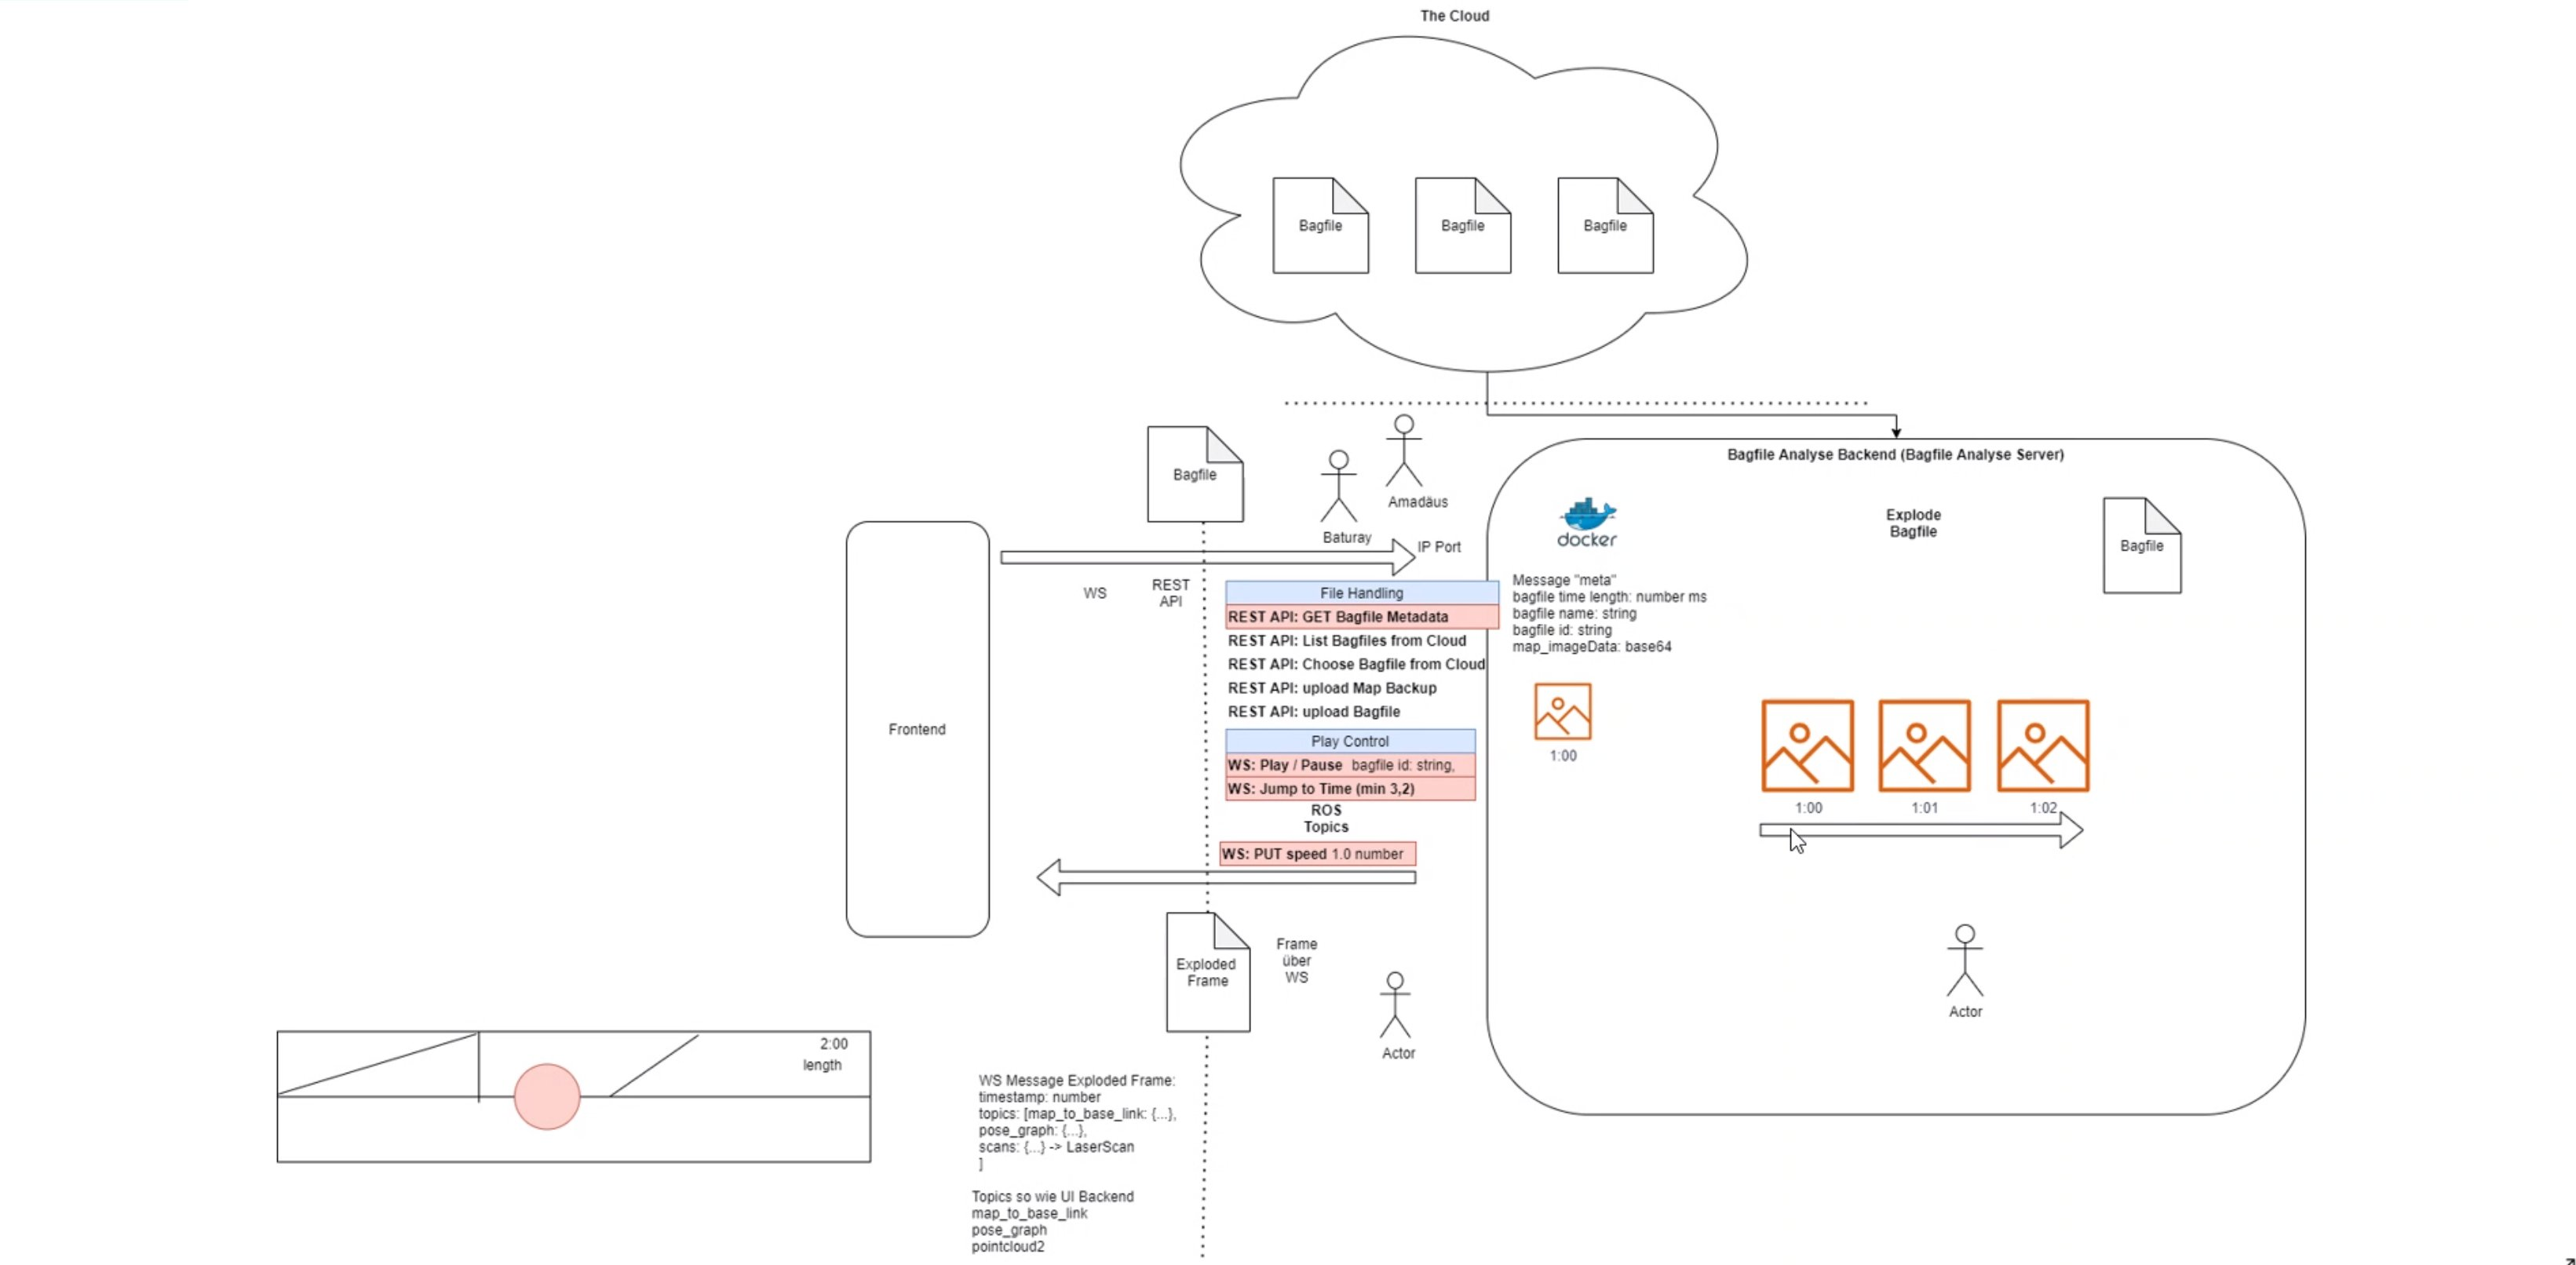
\includegraphics[height=10cm,width=\linewidth]{images/architecture.jpg}
		\caption{Architecture of Rosbag player}
	\end{center}
\end{figure}
\pagebreak
\section{Compare between different libraries}
For implementation of the backend to support rosbag play and every other functionalities python libraries must be used. There were several libraries that can be used to manipulate the rosbag on the backend. 

Basically I did research on sevaral libraries which supports the playing of the rosbag just like command ine used to play the bag.

There were many python libraries which does the same job of playing the rosbag.

\begin{enumerate}
	\item bagpy
	\item rospy
	\item rosbag
	\item pyrosbag
\end{enumerate} 
Some of the libraries which I used is as follows. There were some advantages and disadvantages of libraries.
\begin{enumerate}
	\item bagpy: This library provides a wrapper class call bagreader which is written in python. This provides an easy to use interface for reading rosbag which are recorded by rosbag record command. This library internally uses the rosbag to perform certain operations. 
	
	This library is basically used only to read the topics and there content. But this can't be used to manipulate the bag like playing, recording or anything.

	
	\item rospy: This a python client library for ROS. This client library will quickly enables to interface with ROS Topics, Services and parameters. This enables to access all the information of topics of ROS.
	
	Since we wanted to change the speed of the rosbag on the run time, so this library didn't supported in doing that. Using this library we can only change the speed of the rosbag in the starting of the bag. While running of the bag speed cannot be changed.
	
	\item rosbag: The rosbag package provides the command-line tool for working with bags as well as code APIs for writing and reading bags. This library can't be used to play the rosbag.
	
	\item pyrosbag: This is a library which will create a python library for handling of rosbag. This particular library uses the rosbag and os library to handle all the required functionalities. 
	
	Since the requirement is satisfied with this library we are using pyrosbag library in the backend to support the rosbag part.
\end{enumerate}

\section{Compare between Websockets-API and REST-API} 

In this approach, we needed the communication between the client and server, where the frontend tool will be client and backend tool will be server. So for this hybrid approach to entangle the requirements has been followed. 

\textbf{Websockets:} Websockets is bi-directional communication protocol which enables the continuous communication between the client and server. Since the playing, pausing and stopping of rosbag, stepping of rosbag must via ros-service call, so it must be continuous. Also our future goal is write as well as read ros-topic information. Since in the case of RESt-API it will create instance of that instant and it is not time efficient. Therefore the communication between the frontend and backend for the playing, increasing/decreasing, jumping to time of rosbag part is decided to be via websockets. 
 
\textbf{REST-API:} REST-API is uni-directional communication between server and client. For example in ROS-case we can only read the rostopic information, but we can write or publish to the topic. In some requirements of our project like getting list of bag-files from cloud, choosing which bagfile to be played, uploading the bagfile and uploading the map of factory, it will be one way communication. Either we write a map to cloud, or read the list of the bagfiles in cloud. So for these requirements REST-API is used for communication. 

\section{ROSBRIDGE}
In the frontend codes were implemented in JSON to create the functionalities like connecting pause and play button to the rosservices. Some other functionalities includes integration of slider with jump function.

Since the websocket interface is used for all these functionalities. So we had option of implementing with either os level program or using Rosbridge. Rosbridge provides the JSON API to ROS functionalities.Since the backend works completely with ROS, so Rosbridge is decided as API for frontend. 
 

\section{Concept to visualize the map}

As the rosbag player plays the recorded topic and actions that have been executed on factories. Before implementation of this Rosbag player UI, if the customer gives the rosbag, we will play the rosbag on rviz on our local machines with the arguement of which factories map to be displayed on the rviz background. This basically works by converting the map occupancy grid layer values into real map. Then this values are published in the \textbf{map} topic which enables the rviz to subscribe and visualize it. 

Similar idea is used in this project. So when the customer uploads the map or factory information, the occupancy grid map from backup which is updated frequently is converted to map. Then this will be published in map topic, which is subscribed by rosbridge and converted accordingly to visualize in frontend.
\section{Docker}

To make the current implementation independent of particular OS and make it independent of hardware used. Therefore everything is made compatible with Docker images and containers





	\chapter{Implementation}

With the above described requirements, designs and specification, implementing the first MVP product started. The two teams were involved in the  development of product. One team focused on the development of ROS part required which is backend department. Other team focused on the frontend side of the project that is the UI/UX team. 

I was involved in the backend part of the team. My main goal was to create the services and topics to handling of the rosbag. Handling of the rosbag included like playing, pausing, jumping to the particular location of the rosbag, increasing the speed of the rosbag. With the previous research on the required library it was able to handle the rosbag with the rosservices. 

Some requirements of the project only was needed to be known by the frontend side. For example the duration of the rosbag. So those data are just published by the topic so that on the frontend side it can just be subscribed and get the data. 

Another major task was to create the REST-API for jobs which are not performed continuously and cannot be done only with rosservices. This included the upload of bag to cloud, updating of the map. This also included the downloading of bag from particular http link. The look of REST-API looks as shown in below figure
\begin{figure}[h]
	\begin{center}
		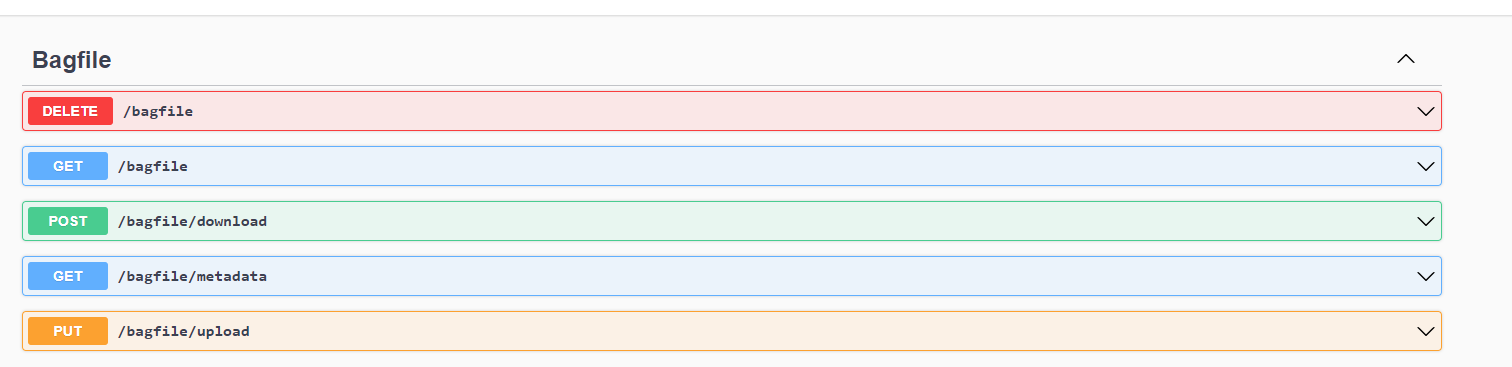
\includegraphics[height=8cm,width=\linewidth]{images/rest-api.png}
		\caption{REST-API endpoints}
	\end{center}
\end{figure}
I tried to implement the above mentioned tasks along with help of my colleagues.
 
Then the communication between the backend and frontend part have been implemted by rossbridge and websockets. Implementation of websockets is just opening of the ports and then waiting for the command to come from frontend. The command from the frontend with comes from the Rosbridge which gives the ROS-API wrapper in json file. I helped in the initial setup of rosbridge and websockets. The small and simple code which is used to test the rosbridge and websockets which is used to communicate between the fronend and backend is shown in below figure.  Then the rest further development of json folder structure is taken care by UI/UX team.
\pagebreak
\begin{figure}[h]
	\begin{center}
		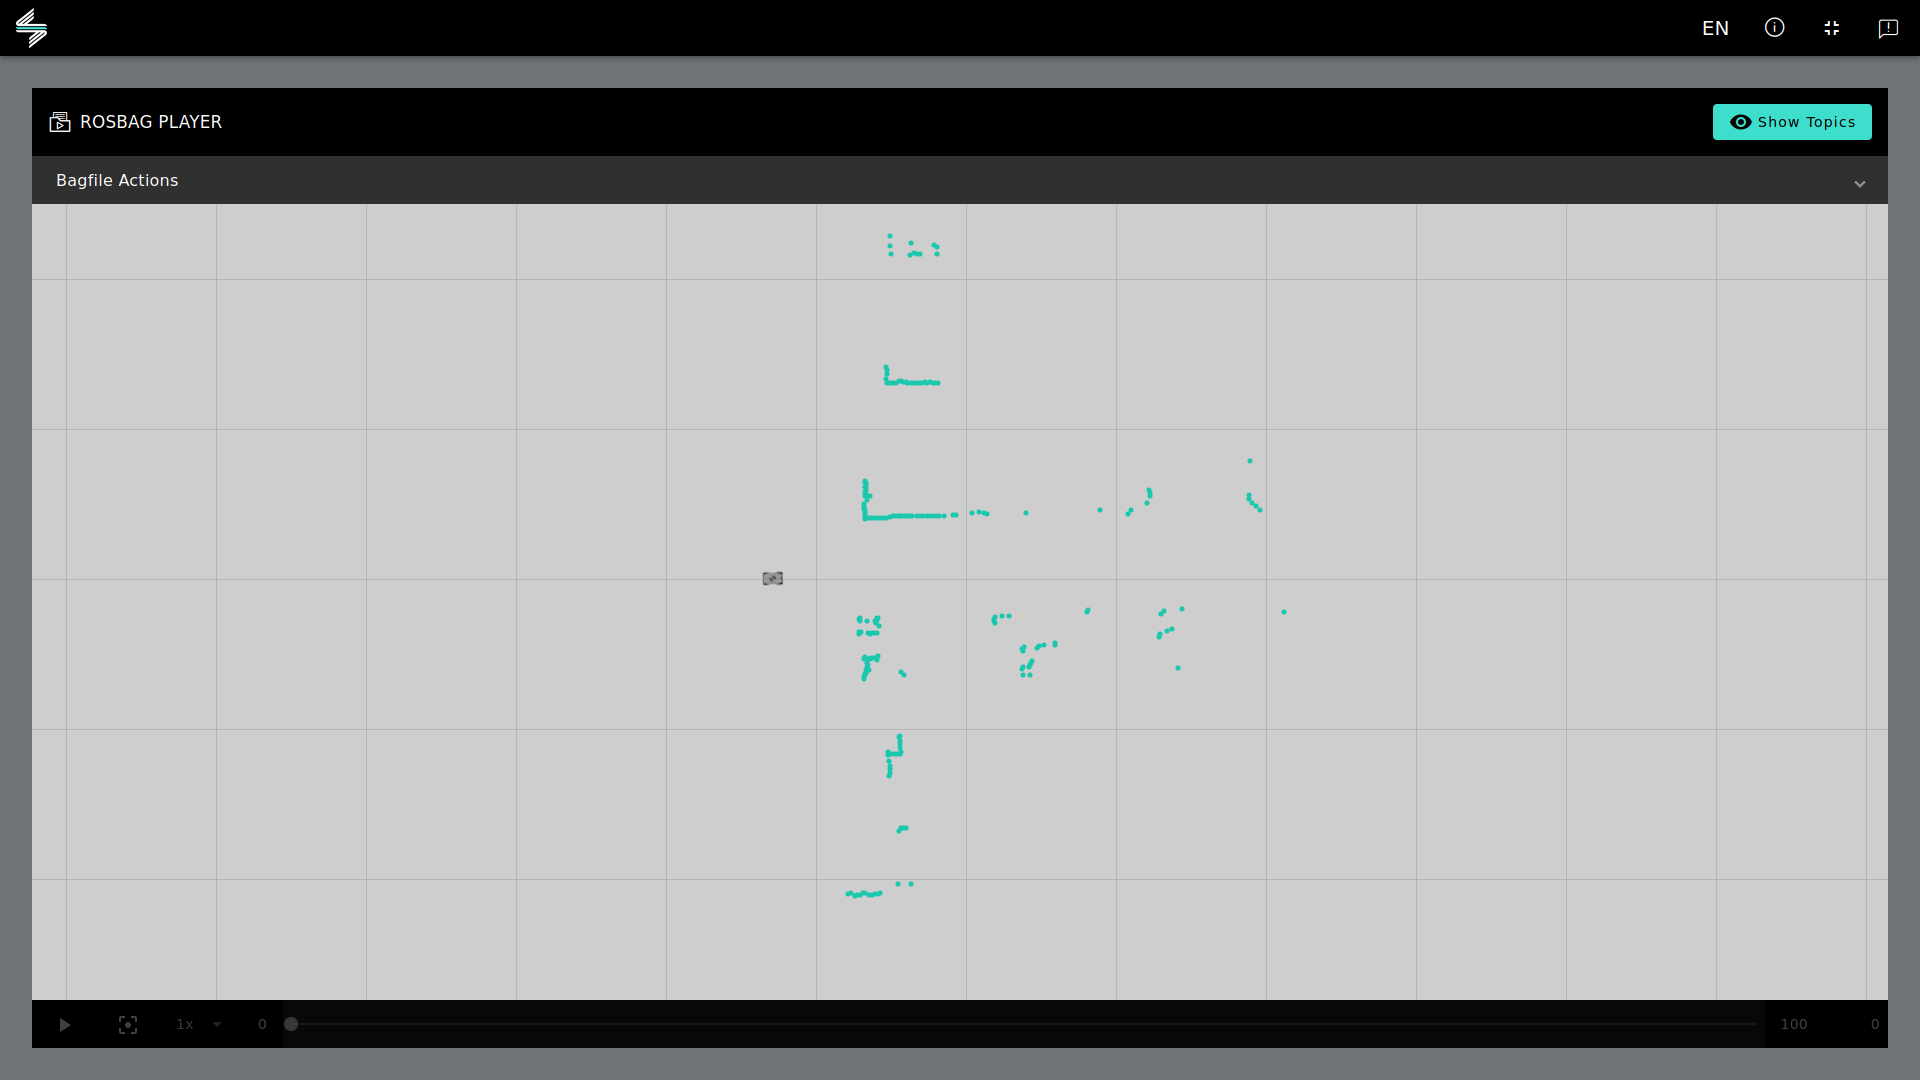
\includegraphics[height=10cm,width=\linewidth]{images/frontend-rosbag.png}
		\caption{Frontend of rosbag player}
	\end{center}
\end{figure}
 
The another task was to make the map visualize in the frontend UI tool. This involved the conversion of occupancy grid to map image. The customer requirement also suggested to find the which version of robot is used based on the file name of the rosbag. This part was implemented by colleagues in the backend team. 

Then the major part of the project, which involved the development of frontend UI for customer. This involved designing the look of the robot, designing of the frontend layouts, subscribing to particular rostopic and analysing and plotting it. All these tasks were done by frontend UI/UX team members.

Currently the functionality of backend is implemented and frontend is able to get some of topics like /odom and all. The buttons for pause/play, slider to jump to particular time, and buttons to change the speed is implemented which will interact with the backend via websockets and rosbridge.The current fronend is as shown in the figure below.
	\chapter{Verification and Validation}
The verification of the code is done in four stages.
\begin{enumerate}
	\item Local verification in PC
	\item Code review
	\item CI/CD
	\item Integration of frontend and backend
\end{enumerate}

\section{Local verification in PC}
Basically basic verification of the code is done on the local PC. This verification of code mainly focuses on the initial implementation and working of the code.
 
\section{Code review}
Every code of this project is maintained as separate repository in the Gitlab of Node robotics. Every tasks are taken into separate branched from the master branch and worked on it. Later if the code is working as required it is then proceeded with merge request process. NODE robotics follows the two-eye review concept, where every merge requests will be verified by the other team members. Everyone are free to give there reviews. Then the given code will be merged to the main branch only if the code gets two approval by other team members. 

This process mainly focuses on the gathering of ideas to solve particular problem in efficient way. Also, includes spelling checks, description checks etc.
\begin{figure}[h]
	\begin{center}
		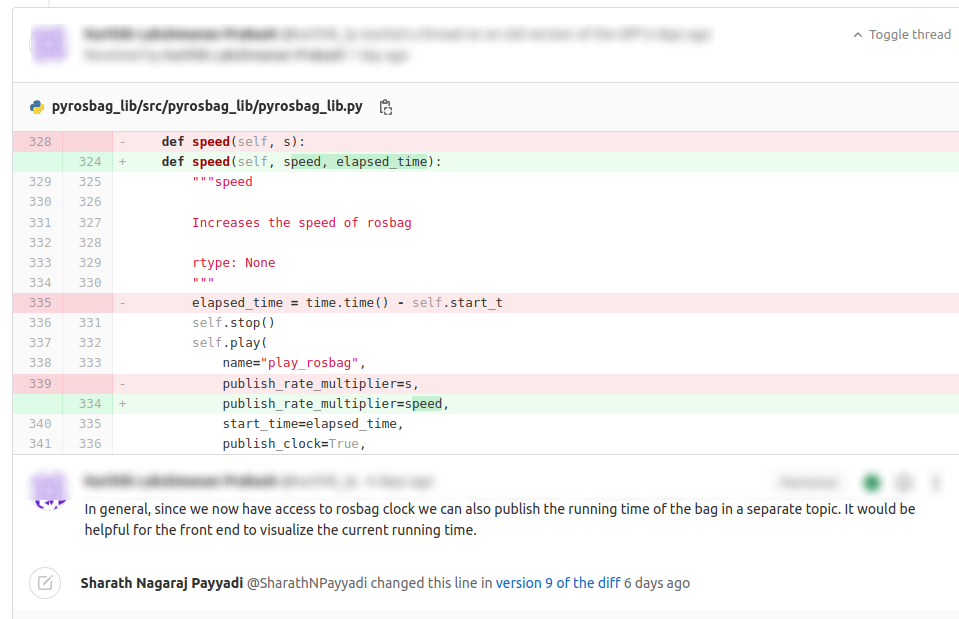
\includegraphics[height=10cm,width=\linewidth]{images/code-review.png}
		\caption{Code review}
	\end{center}
\end{figure}
 
\section{CI/CD}
The third part of verification comes with CI/CD tool. This is tool which enable to integrate our code with companies code. This CI/CD pipeline will be checked once when the merge request is created to the master branch. In this CI/CD tool different jobs have been defined. Some of the jobs are like black, mypy, code\_quality, catkin lint, check suitably for melodic and noetic. For example black will make sure that written python code is universally standard. 

This toll mainly focuses on the improvement of the code quality and versatility of the code. 

\begin{figure}[h]
	\begin{center}
		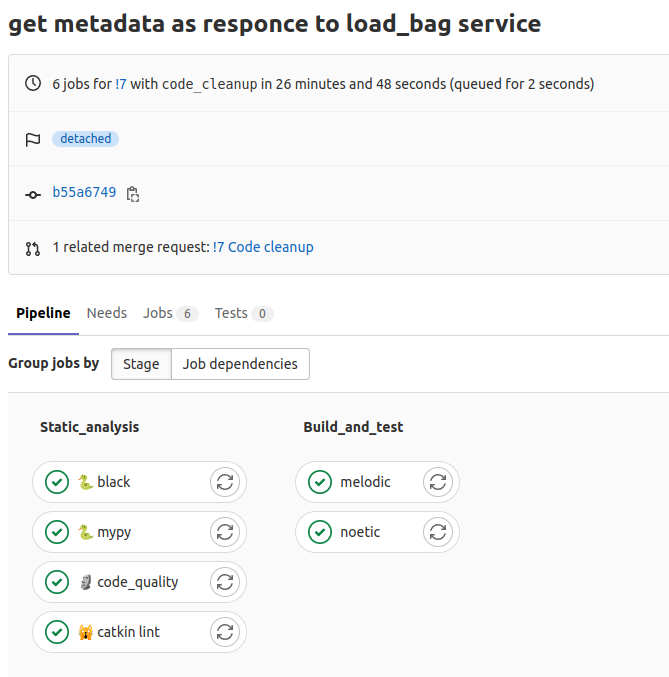
\includegraphics[height=10cm]{images/cicd.png}
		\caption{CI/CD pipelines}
	\end{center}
\end{figure}
\pagebreak
\section{Integration of frontend and backend}
The last part of verification and validation includes the integration of both backend and frontend code. Since the implementation of backend takes place using docker. So we needed to build the image to test the functionality. With the actual implementation we got more reviews. 

This part mainly focuses on the actual working which helps to entangle the future problem
	\chapter{Conclusion and Future scope}
\section{Conclusion}
In this project the UI frontend tool the Rosbag player has been created. The backend part of the product works on python libraries. The communication between fronend and backend has been achieved using websockets and rosbridge. 

During the course of project several issues has been solved. Some of the problem included the tackling of the messages from the topics in frontend tools.

Finally with this tool we can currently look at the metadata like topic list, duration of the rosbag. We can also handle playing of the rosbag like vary the speed, jump to the particular part of the rosbag using slider. We can also analyze the scans that are present on the rosbag. 

\section{Future scope}

This project can further be developed. One of the feature that can be included is the visualization of the map of the manufacturing unit. Also, plotting of the values coming on the ros-topics can definitely one of the interesting feature. 

Another feature that can be implemented like creating the issue on the JIRA board using the frontend tool whenever the error is detected.
	\chapter{References}
\begin{enumerate}
	\item https://node-robotics.com/en/
	\item http://wiki.ros.org/ROS/
	\item http://wiki.ros.org/rosbag
	\item http://library.isr.ist.utl.pt/docs/roswiki/rosbridge.html
	\item https://www.educba.com/websocket-vs-rest/
	\item https://webviz.io/
	\item https://medium.com/cruise/webviz-fb5f77ebe52b
	\item https://docs.docker.com/get-started/overview/
	\item https://bluebotics.com/vda-5050-explained-agv-communication-standard/
	\item https://www.redhat.com/en/topics/devops/what-is-ci-cd
	\item https://en.wikipedia.org/wiki/Autonomous\_robot
	
	
	
	\item https://pypi.org/project/pyrosbag/
	
	
\end{enumerate}
	\chapter{Appendix}
\section{AMR}

AMR's also called as Autonomous mobile robots. It is a robot which acts without the recourse to human control. These mobile robots are majorly used in manufacturing industries. The first autonomous robots environment were known as Elmer and Elsie, which were constructed in the late 1940s by W. Grey Walter. 

The most important feature required for complete physical autonomy is the ability for robot to take care of itself. Some of these robots can be charged by connecting station, few of them have self docking ability. 

Another feature is sensing of environment. The robots should know the place where they exactly located. This is also called as localization. 

\subsection{Autonomous navigation}

For a robot to associate behaviors with a place (localization) requires it to know where it is and to be able to navigate point-to-point.  Such navigation began with wire-guidance in the 1970s and progressed in the early 2000s to beacon-based triangulation. Current commercial robots autonomously navigate based on sensing natural features. At first, autonomous navigation was based on planar sensors, such as laser range-finders, that can only sense at one level. The most advanced systems now fuse information from various sensors for both localization (position) and navigation. Systems such as Motivity can rely on different sensors in different areas, depending upon which provides the most reliable data at the time, and can re-map a building autonomously.

Rather than climb stairs, which requires highly specialized hardware, most indoor robots navigate handicapped-accessible areas, controlling elevators, and electronic doors. With such electronic access-control interfaces, robots can now freely navigate indoors. Autonomously climbing stairs and opening doors manually are topics of research at the current time.

As these indoor techniques continue to develop, vacuuming robots will gain the ability to clean a specific user-specified room or a whole floor. Security robots will be able to cooperatively surround intruders and cut off exits. These advances also bring concomitant protections: robots' internal maps typically permit "forbidden areas" to be defined to prevent robots from autonomously entering certain regions.
	\index{key}
\end{document}